\PassOptionsToPackage{unicode=true}{hyperref} % options for packages loaded elsewhere
\PassOptionsToPackage{hyphens}{url}
%
\documentclass[
  ignorenonframetext,
]{beamer}
\usepackage{pgfpages}
\setbeamertemplate{caption}[numbered]
\setbeamertemplate{caption label separator}{: }
\setbeamercolor{caption name}{fg=normal text.fg}
\beamertemplatenavigationsymbolsempty
% Prevent slide breaks in the middle of a paragraph:
\widowpenalties 1 10000
\raggedbottom
\setbeamertemplate{part page}{
  \centering
  \begin{beamercolorbox}[sep=16pt,center]{part title}
    \usebeamerfont{part title}\insertpart\par
  \end{beamercolorbox}
}
\setbeamertemplate{section page}{
  \centering
  \begin{beamercolorbox}[sep=12pt,center]{part title}
    \usebeamerfont{section title}\insertsection\par
  \end{beamercolorbox}
}
\setbeamertemplate{subsection page}{
  \centering
  \begin{beamercolorbox}[sep=8pt,center]{part title}
    \usebeamerfont{subsection title}\insertsubsection\par
  \end{beamercolorbox}
}
\AtBeginPart{
  \frame{\partpage}
}
\AtBeginSection{
  \ifbibliography
  \else
    \frame{\sectionpage}
  \fi
}
\AtBeginSubsection{
  \frame{\subsectionpage}
}
\usepackage{lmodern}
\usepackage{amssymb,amsmath}
\usepackage{ifxetex,ifluatex}
\ifnum 0\ifxetex 1\fi\ifluatex 1\fi=0 % if pdftex
  \usepackage[T1]{fontenc}
  \usepackage[utf8]{inputenc}
  \usepackage{textcomp} % provides euro and other symbols
\else % if luatex or xelatex
  \usepackage{unicode-math}
  \defaultfontfeatures{Scale=MatchLowercase}
  \defaultfontfeatures[\rmfamily]{Ligatures=TeX,Scale=1}
\fi
\usetheme[]{Malmoe}
% use upquote if available, for straight quotes in verbatim environments
\IfFileExists{upquote.sty}{\usepackage{upquote}}{}
\IfFileExists{microtype.sty}{% use microtype if available
  \usepackage[]{microtype}
  \UseMicrotypeSet[protrusion]{basicmath} % disable protrusion for tt fonts
}{}
\makeatletter
\@ifundefined{KOMAClassName}{% if non-KOMA class
  \IfFileExists{parskip.sty}{%
    \usepackage{parskip}
  }{% else
    \setlength{\parindent}{0pt}
    \setlength{\parskip}{6pt plus 2pt minus 1pt}}
}{% if KOMA class
  \KOMAoptions{parskip=half}}
\makeatother
\usepackage{xcolor}
\IfFileExists{xurl.sty}{\usepackage{xurl}}{} % add URL line breaks if available
\IfFileExists{bookmark.sty}{\usepackage{bookmark}}{\usepackage{hyperref}}
\hypersetup{
  pdftitle={The Gibbs Sampler},
  pdfauthor={M Loecher},
  pdfborder={0 0 0},
  breaklinks=true}
\urlstyle{same}  % don't use monospace font for urls
\newif\ifbibliography
\setlength{\emergencystretch}{3em}  % prevent overfull lines
\providecommand{\tightlist}{%
  \setlength{\itemsep}{0pt}\setlength{\parskip}{0pt}}
\setcounter{secnumdepth}{-2}

% set default figure placement to htbp
\makeatletter
\def\fps@figure{htbp}
\makeatother



\definecolor{fsblue}{RGB}{0, 72, 128}
\definecolor{fsblue}{RGB}{54,66,109}
\definecolor{lightgrey}{RGB}{245,245,245}
\definecolor{mygrey}{RGB}{230,230,230}
\setbeamercolor{author in head/foot}{bg=fsblue}
%\setbeamercolor{title in head/foot}{bg=fsblue}
%\setbeamercolor{title in head/foot}{bg=white,fg=darkblue}
%\setbeamercolor{author in head/foot}{bg=white,fg=darkblue}
%\setbeamerfont{frametitle}{size=\large,series=\bfseries}
%\setbeamercolor{frametitle}{fg=darkred}
%
%\setbeamerfont{block title}{size=\normalsize,series=\bfseries}
%\setbeamertemplate{blocks}[rounded][shadow=true]
%\setbeamercolor{block body}{bg=lightgrey}
%\setbeamercolor{block title}{bg=mygrey,fg=black}
%
%%\setbeamersize{text margin left=1.5cm,text margin right=1.5cm} 
%\setbeamerfont*{itemize/enumerate subbody}{parent=itemize/enumerate body}
%\setbeamerfont*{itemize/enumerate subsubbody}{parent=itemize/enumerate
%  body}

\usepackage{color}
\usepackage{setspace}
%\setstretch{1.25}
\setstretch{1.15}
\usepackage{slashbox}
\usepackage{hyperref}
\usepackage{graphics}
%\usepackage{fancybox}
\usepackage{amsmath,amsthm,bm}
%\usepackage[longnamesfirst]{natbib}
\usepackage{natbib}
\bibpunct{(}{)}{;}{a}{,}{,}

%\usepackage[makestderr]{pythontex}

\definecolor{markergreen}{rgb}{0.6, 1.0, 0}
\definecolor{darkred}{rgb}{.7,0,0}
\providecommand{\marker}[1]{\fcolorbox{markergreen}{markergreen}{{#1}}}
\providecommand{\natp}[1]{\textcolor{darkred}{#1}}


%%%%%%%%%%%%%%%%%%%%%%%%%%%%%%%%%%%%%%%%%%%%%%%%%%%%%%%%%%
%
%  Reset some default colors for itemize/enumerate/description environments
%
\setbeamercolor{description item}{fg=darkred!80!black}  %  Color of key word in desciption 
%\setbeamercolor{alerted text}{fg=darkred!80!black}  %  Color of key word in desciption 
\setbeamercolor{alerted text}{fg=darkblue}  %  Color of key word in desciption 
%
\definecolor{darkred}{rgb}{0.7,0,0}
\definecolor{darkgreen}{rgb}{0,0.6,0}
\setbeamercolor{item}{fg=darkgreen}  %  The dot color
\definecolor{darkblue}{rgb}{0,0,0.8}
\setbeamercolor{itemize/enumerate body}{fg=black}    % Text Level 1
%\setbeamercolor{itemize/enumerate subbody}{fg=darkblue}    % Text Level 2
\setbeamercolor{itemize/enumerate subsubbody}{fg=green!25!black}    % Text Level 3

\setbeamertemplate{headline}{}

\definecolor{grey}{RGB}{.25,.0,.25}
%\definecolor{fsblue}{rgb}{0, 0, 1}

%\setbeamerfont{note page}{size=\footnotesize}
%\setbeamercolor{math text}{fg=darkblue}
%\setbeamercolor{math text displayed}{fg=darkblue}
%
%\providecommand{\mgreenbox}[1]{\fcolorbox{green}{green}{$#1$}}
%\providecommand{\mredbox}[1]{\fcolorbox{red}{white}{$#1$}}
%\providecommand{\mredblockbox}[1]{\fcolorbox{red}{blocktitle.bg!.0!bg}{$#1$}}
%\providecommand{\mbluebox}[1]{\fcolorbox{blue}{white}{$#1$}}
%\providecommand{\mwhitebox}[1]{\fcolorbox{white}{white}{$#1$}}
%\providecommand{\hyperl}[2]{\textcolor{blue}{\hyperlink{#1}{#2}}}
%\providecommand{\Nzero}{\mathbb N_0}
%
%\providecommand{\bluebox}[1]{\text{\fcolorbox{blue!10}{blue!10}{#1}}}  
%\providecommand{\redbox}[1]{\text{\fcolorbox{red!15}{red!15}{#1}}}  
%\providecommand{\greenbox}[1]{\text{\fcolorbox{darkgreen!15}{darkgreen!15}{#1}}}  
%
%\providecommand{\limc}{\ensuremath{\lim_{C\rightarrow-\infty}}}
%\providecommand{\limcp}{\ensuremath{\lim_{C\rightarrow\infty}}}
%\providecommand{\ct}{\ensuremath{\cos \theta}}
%\providecommand{\st}{\ensuremath{\sin \theta}}
%\providecommand{\cp}{\ensuremath{\cos \varphi}}
%\renewcommand{\sp}{\ensuremath{\sin \varphi}}
\usepackage{multirow}

\usepackage{mathrsfs}

%% GENERAL DEFINITIONS
\unitlength1cm

%% COMMAND DEFINITIONS
\newcommand{\E}{{\mathbb{E}}}
%%\renewcommand{\E}{{\mathds E}}
%%\renewcommand{\E}{{\varmathbb{E}}}
%%\renewcommand{\E}{{\mathrm{I\!E}}}
\providecommand{\R}{{\mathbb{R}}}
\newcommand{\T}{{\mathbb{T}}}
\newcommand{\Fb}{{\mathbb{F}}}
\newcommand{\Eqn}{{\mathbb{E}}_{{\bf Q}_N}}
\newcommand{\Eq}{{\mathbb{E}}_{{\bf Q}}}
\newcommand{\Eqm}{{\mathbb{E}}_{{\bf Q}_M}}
\newcommand{\EqT}{{\mathbb{E}}_{{\bf Q}_T}}
\newcommand{\EqTz}{{\mathbb{E}}_{{\bf Q}_{T_2}}}
\newcommand{\EqTe}{{\mathbb{E}}_{{\bf Q}_{T_1}}}
\newcommand{\EqSe}{{\mathbb{E}}_{{\bf Q}_{S^1}}}
\newcommand{\EqSz}{{\mathbb{E}}_{{\bf Q}_{S^2}}}
\newcommand{\p}{{\bf P}}
%%%
%% $Id: definitions.tex,v 1.3 2009/12/06 12:46:09 natalie Exp $
%% $Source: /Users/natalie/cvs/tex/stressed/definitions.tex,v $
%% $Date: 2009/12/06 12:46:09 $
%% $Revision: 1.3 $
%%

\usepackage{mathrsfs}

%% GENERAL DEFINITIONS
\unitlength1cm

%% COMMAND DEFINITIONS
\newcommand{\E}{{\mathbb{E}}}
%%\renewcommand{\E}{{\mathds E}}
%%\renewcommand{\E}{{\varmathbb{E}}}
%%\renewcommand{\E}{{\mathrm{I\!E}}}
\providecommand{\R}{{\mathbb{R}}}
\newcommand{\T}{{\mathbb{T}}}
\newcommand{\Fb}{{\mathbb{F}}}
\newcommand{\Eqn}{{\mathbb{E}}_{{\bf Q}_N}}
\newcommand{\Eq}{{\mathbb{E}}_{{\bf Q}}}
\newcommand{\Eqm}{{\mathbb{E}}_{{\bf Q}_M}}
\newcommand{\EqT}{{\mathbb{E}}_{{\bf Q}_T}}
\newcommand{\EqTz}{{\mathbb{E}}_{{\bf Q}_{T_2}}}
\newcommand{\EqTe}{{\mathbb{E}}_{{\bf Q}_{T_1}}}
\newcommand{\EqSe}{{\mathbb{E}}_{{\bf Q}_{S^1}}}
\newcommand{\EqSz}{{\mathbb{E}}_{{\bf Q}_{S^2}}}
\newcommand{\p}{{\bf P}}
%\renewcommand{\p}{\ensuremath{\mathbb{P}}}
%%\renewcommand{\p}{{\mathds{P}}}
%%\renewcommand{\p}{{\varmathbb{P}}}
%%\renewcommand{\p}{{\mathrm{I\!P}}}
\newcommand{\pas}{\text{{\bf P}--a.s.}}
\renewcommand{\pas}{\ensuremath{\mathbb{P}\text{--a.s.}}}
\newcommand{\paa}{\text{{\bf P}--a.a.}}
\renewcommand{\paa}{\ensuremath{\mathbb{P}\text{--a.a.}}}
\newcommand{\qas}{\text{{\bf Q}--a.s.}}
\renewcommand{\qas}{\ensuremath{\mathbb{Q}\text{--a.s.}}}

%\newcommand{\e}{{\bf e}}
\newcommand{\e}{\ensuremath{e}}
\newcommand{\q}{{\bf Q}}
\renewcommand{\q}{\ensuremath{\mathbb{Q}}}
\newcommand{\qn}{{\bf Q}_N}
\newcommand{\qm}{{\bf Q}_M}
\newcommand{\qT}{{\bf Q}_T}
\newcommand{\qTz}{{\bf Q}_{T_2}}
\newcommand{\qTe}{{\bf Q}_{T_1}}
\newcommand{\qS}{{\bf Q}_S}
\newcommand{\qSe}{{\bf Q}_{S^1}}
\newcommand{\qSz}{{\bf Q}_{S^2}}
\newcommand{\F}{{\cal F}}
\newcommand{\G}{{\cal G}}
\newcommand{\A}{{\cal A}}
\newcommand{\Hc}{{\cal H}}
\newcommand{\dP}{{\rm d}{\bf P}}
\newcommand{\du}{{\rm d}u}
%%\newcommand{\dt}{{\rm d}t}
\newcommand{\dd}{{\rm d}}
\newcommand{\df}{{\rm \bf DF}}
\providecommand{\N}{{\mathbb N}}
\providecommand{\Ncdf}{{\rm N}}
\newcommand{\n}{{\rm n}}
\newcommand{\emb}{\bf \em}
\newcommand{\1}{\ensuremath{\mathbf{1}}}
\newcommand{\qs}{{\q_{\rm Swap}}}
\newcommand{\fx}{{\rm fx}}
\newcommand{\V}{{\rm Var}}
%\newcommand{\C}{{\bf C}}
\newcommand{\Om}{{\Omega}}
\providecommand{\limn}{\ensuremath{\lim_{n\rightarrow\infty}}}
\providecommand{\qv}[2]{\ensuremath{\langle #1,#1\rangle_{#2}}}

%% ENVIRONMENT DEFINITIONS
%\newtheorem{prop}{Proposition}[section]
%\newtheorem{theo}{Theorem}[section]
%\newtheorem{lem}{Lemma}[section]
%\newtheorem{ass}{Assumption}[section]
%\newtheorem{cor}{Corollary}[section]
%\newtheorem{aufg}{Exercise}[section]
%\newtheorem{defi}{Definition}[section]

\ifx\prop\undefined
\newtheorem{prop}{Proposition}[section]
\fi
\newtheorem{theo}[prop]{Theorem}
\newtheorem{lem}[prop]{Lemma}
\newtheorem{cor}[prop]{Corollary}
\newtheorem{defi}[prop]{Definition}

%% enumeration in lists
\providecommand{\labelenumi}{{\rm (\roman{enumi})}}
   %\setlength{\topsep}{0cm}
    \setlength{\labelsep}{0.3cm}
    %\setlength{\itemindent}{0cm}
   \setlength{\leftmargin}{10cm}
    \setlength{\labelwidth}{5cm}

\providecommand{\cadlag}{c\`adl\`ag }
\providecommand{\cadlagns}{c\`adl\`ag}
\providecommand{\caglad}{c\`agl\`ad }
\providecommand{\cad}{c\`ad}
\providecommand{\cag}{c\`ag}
\providecommand{\levy}{L\'evy\ }
\providecommand{\levyns}{L\'evy}
\providecommand{\levyito}{L\'evy-It\^o\ } 
\providecommand{\levykhinchin}{L\'evy-Khinchin\ }
\providecommand{\D}{\ensuremath{D(\R_+,\R)}}
\providecommand{\Dsig}{\ensuremath{D(\R_+, \R_+\setminus\{0\}})}
\providecommand{\Dd}{\ensuremath{D(\R_+,\R^d)}}
\providecommand{\C}{\ensuremath{C(\R_+,\R)}}
\providecommand{\Cd}{\ensuremath{C(\R_+,\R^d)}}
\providecommand{\rpos}{\ensuremath{{[0,\infty)}}}
\providecommand{\esup}{\mbox{ess sup}}
\providecommand{\einf}{\mbox{ess inf}}
\def\Z{{\mathbb Z}}
%\def\N{{\mathbb N}}
%\def\R{{\mathbb R}}
%\def\C{{\mathbb C}}
%\def\H{{\mathbb H}}
\def\P{{\mathbb P}}
\def\Q{{\mathbb Q}}
%\def\E{{\mathbb E}}
\def\I{{\mathbb I}}
%\def\T{{\mathbb T}}
%\def\F{{\mathbb F}}
\def\M{{\mathbb M}}
%\def\Hc{{\mathcal H}}
\def\Mc{{\mathcal M}}
\def\filtration#1{{\ensuremath\mathcal{#1}}}
%\def\filt{{\mathcal F}}
\def\tp{\tilde{\p}}
\providecommand{\vec}[1]{\ensuremath{\bm #1}}
\providecommand{\vecb}[1]{\ensuremath{\bm #1}}
\providecommand{\abs}[1]{\ensuremath{\lvert#1\rvert}}
\providecommand{\norm}[1]{\ensuremath{\lVert#1\rVert}}
\providecommand{\var}{\ensuremath{{\rm Var}}}
\providecommand{\cov}{\ensuremath{{\rm Cov}}}
\providecommand{\borel}[0]{\ensuremath{\mathcal{B}}}
\providecommand{\intinf}[0]{\ensuremath{\int_{-\infty}^\infty}}
\providecommand{\intpos}[0]{\ensuremath{\int_0^\infty}}
\providecommand{\intneg}[0]{\ensuremath{\int_{-\infty}^0}}
\providecommand{\todo}[1]{\footnote{#1}}
\providecommand{\dynkin}[0]{\ensuremath{\mathcal D}}
\providecommand{\ce}[2]{\ensuremath{\E(#1|\filtration{#2})}}
\providecommand{\inv}[1]{\ensuremath{#1^{(-1)}}}
\providecommand{\os}[2]{\ensuremath{#1^{(#2)}}}
\providecommand{\pos}[2]{\ensuremath{h_{#1}(#2)}}
%\providecommand{\poslong}[2]{\ensuremath{h(#1, #2)}}
\providecommand{\poslong}[3]{\ensuremath{h_{#1, #2}(#3)}}

\providecommand{\hr}{\ensuremath{{\rm HR}}}
\providecommand{\hc}{\ensuremath{{\rm HC}}}
\providecommand{\vatr}{\ensuremath{{\rm VaR}}}
\providecommand{\ahr}{\ensuremath{{\rm AHR}}}
\providecommand{\es}{\ensuremath{{\rm ES}}}
%% Class of finite variation processes
\providecommand{\classfv}{\ensuremath{\mathscr V}}
\providecommand{\classv}{\ensuremath{\mathscr V}}
%% Stochastic integral operator
\providecommand{\stint}{\ensuremath{\cdotp}}
\providecommand{\classh}{\ensuremath{\mathscr H^2}}
\providecommand{\classhloc}{\ensuremath{\mathscr H^2_{\rm loc}}}
\providecommand{\classm}{\ensuremath{\mathscr M}}
\providecommand{\classmloc}{\ensuremath{\mathscr M_{\rm loc}}}
\providecommand{\classl}{\ensuremath{L^2}}
\providecommand{\classlloc}{\ensuremath{L^2_{\rm loc}}}
\providecommand{\classa}{\ensuremath{\mathscr A}}
\providecommand{\classaloc}{\ensuremath{\mathscr A_{\rm loc}}}
\providecommand{\classalocpos}{\ensuremath{\mathscr A_{\rm loc}^+}}
\providecommand{\classp}{\ensuremath{\mathscr P}}
\providecommand{\classo}{\ensuremath{\mathscr O}}
\providecommand{\classs}{\ensuremath{\mathscr S}}
\providecommand{\classsp}{\ensuremath{\mathscr S_p}}
\providecommand{\nullset}{\ensuremath{\mathscr N}}

\providecommand{\ito}{It\^o }
\providecommand{\itos}{It\^o's\, }

\providecommand{\variation}[2]{\ensuremath{\rm V_{#1}(#2)}}
\renewcommand{\H}{\ensuremath{\mathcal H}}
%% CPO distribution
\providecommand{\cpo}{\ensuremath{{\rm CPO}}}
\providecommand{\Fsigma}{\ensuremath{\mathcal \F_\infty^\sigma}}
\providecommand{\sigd}{\ensuremath{\mathscr D}}

%% Credit spreads
\providecommand{\s}{{\bf s}}
\providecommand{\classu}{\ensuremath{\mathscr U}}

\providecommand{\sX}{\ensuremath{\mathcal X}}
\providecommand{\sY}{\ensuremath{\mathcal Y}}
\providecommand{\dx}{\ensuremath{\frac{\partial}{\partial x}}} %%
\providecommand{\ddx}{\ensuremath{\frac{\partial^2}{\partial^2 x}}} %%
\providecommand{\ddt}{\ensuremath{\frac{\partial^2}{\partial^2 t}}} %%
\providecommand{\dt}{\ensuremath{\frac{\partial}{\partial t}}} %%
\providecommand{\dy}{\ensuremath{\frac{\partial}{\partial y}}} %%
\providecommand{\frechet}{Fr\'echet } %
\providecommand{\frechetns}{Fr\'echet} %
\providecommand{\mda}{\ensuremath{\text{MDA}}} %
\DeclareMathOperator*{\esssup}{ess\,sup}

%\DeclareMathSizes{14.4}{15}{7}{7}

\title{The Gibbs Sampler}
\subtitle{Bayesian Statistics Explorations}
\author{M Loecher}
\date{}

\begin{document}
\frame{\titlepage}

\begin{frame}
  \tableofcontents[hideallsubsections]
\end{frame}
\hypertarget{motivation}{%
\section{Motivation}\label{motivation}}

\begin{frame}{Rejection Sampling}
\protect\hypertarget{rejection-sampling}{}

Last week we learned about a ``general workhorse'' MCMC algorithm, the
\textit{Metropolis Hastings Algorithm}. While it is a powerful and
versatile ``hill climbing'' sampling scheme, there are a few challenges:

\begin{itemize}
  \item Designing a proposal distribution can be tricky
  \item Tradeoff between bandwidth and sampling efficiency (number of rejected samples)
  \item Hyperparameter tuning
\end{itemize}

\end{frame}

\begin{frame}{Hierarchical Models}
\protect\hypertarget{hierarchical-models}{}

Gibbs sampling is another MCMC method which works if all conditional
posterior densities can be explicitly derived.

\begin{itemize}
  \item No specially designed proposal distributions 
  \item No rejected samples
  \item No hyperparameter tuning
  \item Conditionals eays for most hierarchical models
  \item Very popular in machine learning, e.g. LDA, Bayesian Networks, NLP 
\end{itemize}

\end{frame}

\hypertarget{estimation}{%
\section{Estimation}\label{estimation}}

\begin{frame}{Maximum Likelihood}
\protect\hypertarget{maximum-likelihood}{}

Let's say I've flipped a coin \(10\) times and got \(6\) heads, \(4\)
tails. Each coin flip is independent so the likelihood of a value of
\(\theta\) given our observed data is: \[
P(X_1 = x_1, \ldots ,X_{10} = x_{10}) = L(\theta) = \prod_{i=1}^{10}{\theta^{x_i} (1-\theta)^{1-x_i}} = \theta^{6} (1-\theta)^{4}
\]

\begin{center}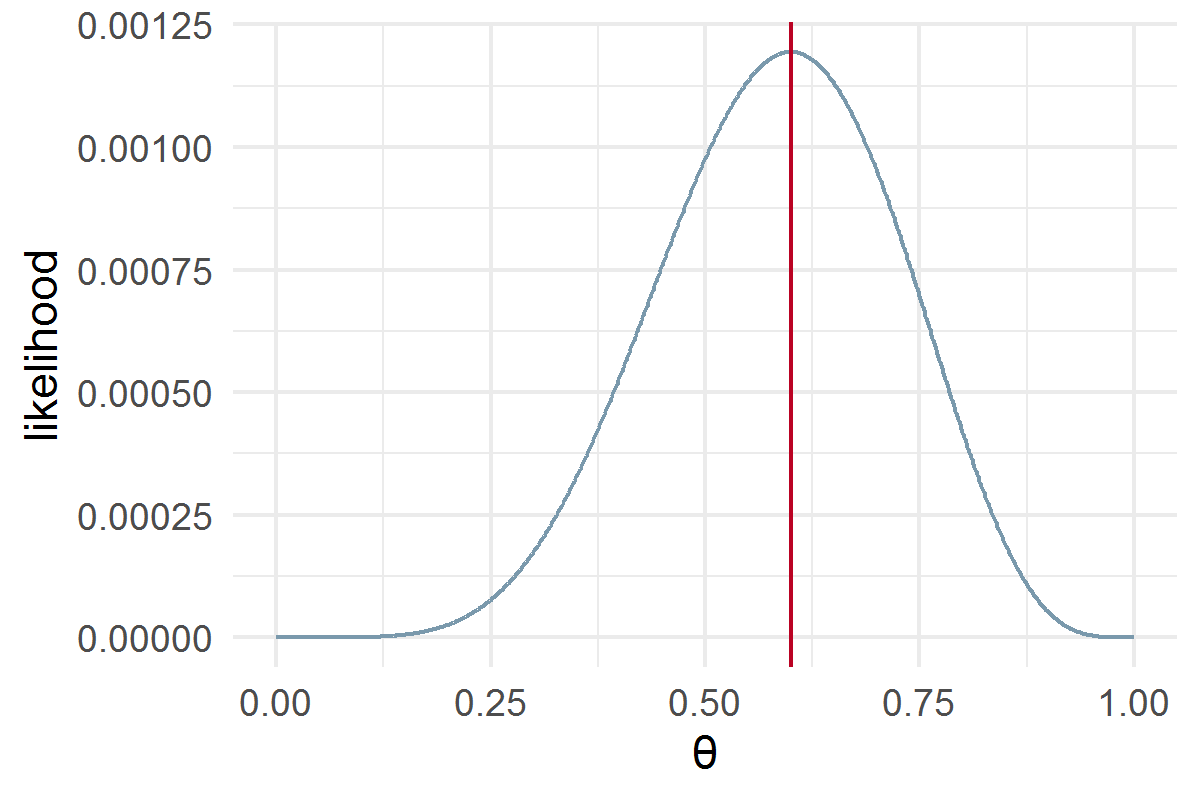
\includegraphics[width=6cm,height=4cm]{figures/LikelihoodCoin} \end{center}

\end{frame}

\begin{frame}{Beta Binomial 1}
\protect\hypertarget{beta-binomial-1}{}

\begin{equation}
\underbrace{p(\theta|D)}_{posterior} = {\overbrace{p(D|\theta)}^{likelihood}
  \overbrace{p(\theta)}^{prior} \over \underbrace{p(D)}_{evidence}}
\end{equation}

\begin{equation}
\underbrace{p(\theta|D)}_{posterior}  \propto  {\overbrace{p(D|\theta)}^{likelihood}
  \overbrace{p(\theta)}^{prior}}
\end{equation}

To estimate the posterior of the bernoulli distribution we plug in our
likelihood and prior (Beta distribution)

\end{frame}

\begin{frame}{Bayesian Estimate}
\protect\hypertarget{bayesian-estimate}{}

The Beta distribution is a conjugate distribution of the binomial
distribution.

\[
\pi(\theta | \alpha, \beta) = Beta(\alpha, \beta) = \theta^{\alpha-1} \cdot (1-\theta)^{\beta-1}/B(\alpha, \beta)
\]

\begin{center}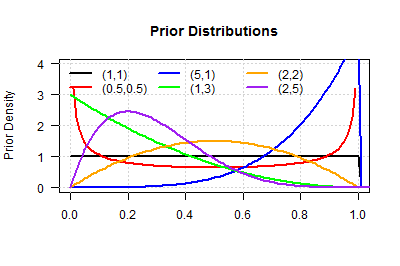
\includegraphics[width=8cm,height=6cm]{figures/BetaPriors} \end{center}

\end{frame}

\begin{frame}{Beta Binomial 2}
\protect\hypertarget{beta-binomial-2}{}

\begin{equation}
p(\theta|z,N) \propto \overbrace{\theta^z(1-\theta)^{(N-z)}}^{likelihood} \overbrace{{\theta^{(\alpha-1)}(1-\theta)^{(\beta-1)}}\over B(\alpha,\beta)}^{prior}
\end{equation}

\begin{equation}
\begin{aligned}
p(\theta|z,N) &\propto {\overbrace{\theta^{(\alpha + z -1)}(1-\theta)^{(N-z+\beta-1)}}^{Same \hspace{1 mm} Pattern \hspace{1 mm} as \hspace{1 mm} Prior}\over{B(\alpha,\beta)}}\\
p(\theta|z,N) &\propto Beta(\alpha+z, N-z+\beta)
\end{aligned}
\end{equation}

\end{frame}

\begin{frame}{Posterior Density}
\protect\hypertarget{posterior-density}{}

Choose a ``weakly informative'' prior: \(\alpha=\beta=2\); Weighted
Average of prior and data based likelihood!
\[\hat{\theta} = \frac{6+2}{10+4}\]

\begin{center}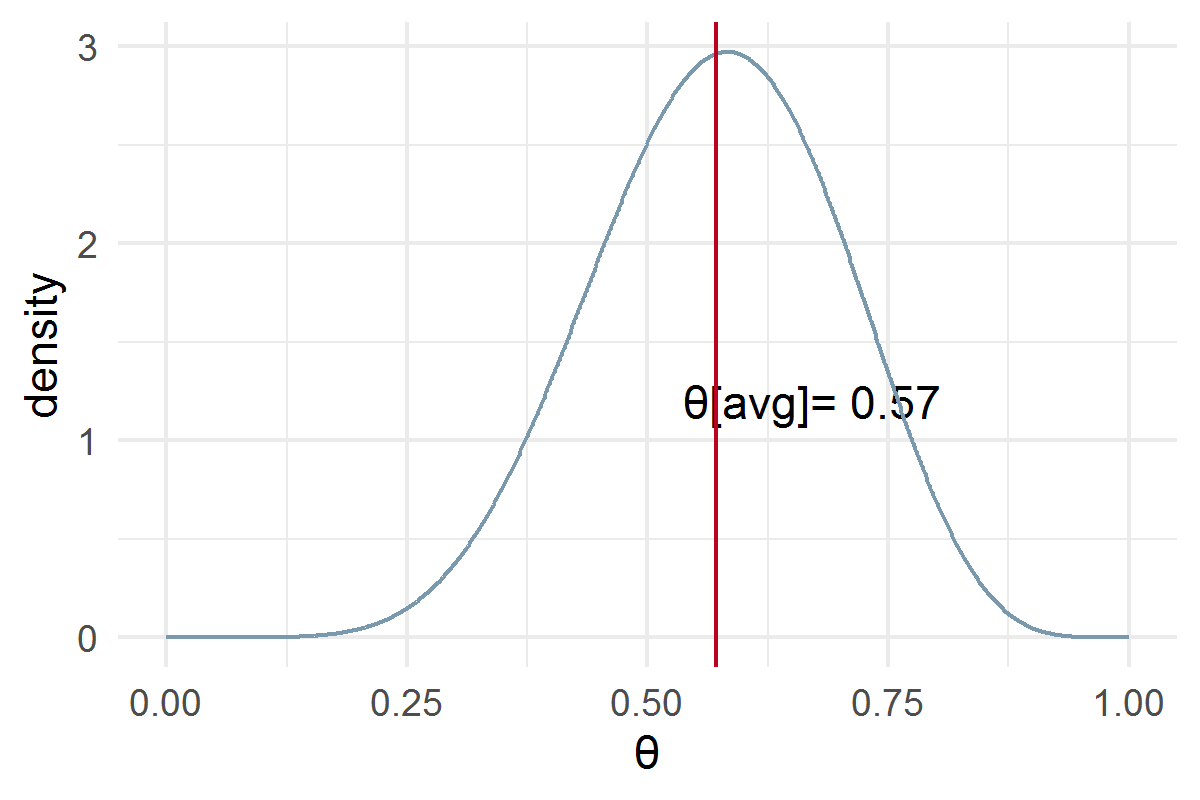
\includegraphics[width=6cm,height=4cm]{figures/PosteriorBeta} \end{center}

\end{frame}

\begin{frame}{Sampling = Estimating}
\protect\hypertarget{sampling-estimating}{}

The coin flip example solved via Bayesian inference was capable of being
solved analytically. However in many cases of Bayesian inference this is
not possible due to the intractability of solving for the marginal
likelihood (evidence term). Imagine we could sample from the posterior:

\begin{center}\includegraphics[width=6cm,height=4cm]{GibbsSampler_files/figure-beamer/unnamed-chunk-5-1} \end{center}

\end{frame}

\begin{frame}{Change Point Example}
\protect\hypertarget{change-point-example}{}

\footnotesize

What if the problem we are solving is more complicated? Let's say I flip
a coin repeatedly, but at some point I switch to another coin with a
different bias \((\theta)\). I want to detect the point in time when
coin 1 was swapped out for coin 2.

\begin{center}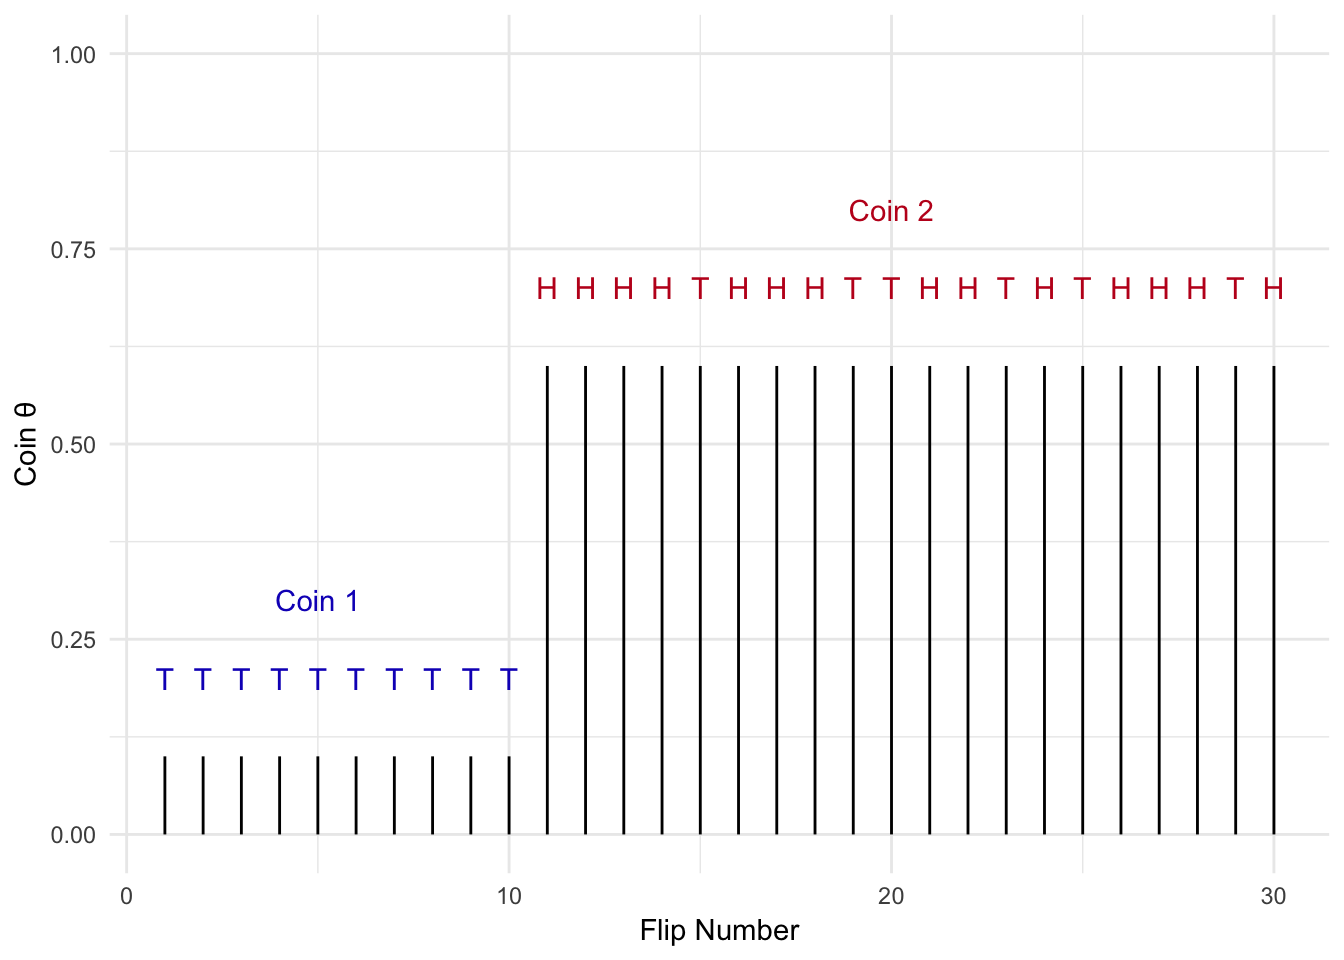
\includegraphics[width=8cm,height=6cm]{figures/ldaFig2_15_bernChangePointExampleFig-1} \end{center}

\end{frame}

\begin{frame}{Generative Model}
\protect\hypertarget{generative-model}{}

\footnotesize

In this case we have 3 variables that we need to estimate:

\begin{enumerate}
  \item Coin bias for coin 1: $\theta_1$
  \item Coin bias for coin 2: $\theta_2$
  \item The point in time, i.e. on which flip, the coin was swapped: $n$
\end{enumerate}

We assume that all values of n are equally probable and therefore can be
modeled as a uniform distribution.

\begin{equation}
\begin{aligned}
  x &\sim   
  \begin{cases}
      Bern(x_{i};\theta_{1}) \quad 1 \le i \le n \\
      Bern(x_{i};\theta_{2}) \quad n < i < N  
  \end{cases} \\
  n &\sim Uniform(2...N) \\
  \theta_{i} &\sim Beta(\theta_{i}, \alpha_i,\beta_i)
\end{aligned}
\end{equation}

\end{frame}

\begin{frame}{Joint Distribution}
\protect\hypertarget{joint-distribution}{}

\footnotesize

\begin{equation}
p(\theta_{1}, \theta_{2}, n| x_{1:N}) \propto \overbrace{p(x_{1:n}|\theta_{1},n)
p(x_{n+1:N}|\theta_{2},n)}^{Likelihoods}
\overbrace{p(\theta_{1})p(\theta_{2})p(n)}^{Priors}
\end{equation}

\begin{equation}
\label{eq:ChgPtJoint}
\begin{aligned}
p(\theta_{1}, \theta_{2}, n| x_{1:N}) &\propto 
  \prod_{1}^{n}p(x_{i}|\theta_{1})
  \prod_{n+1}^{N}p(x_{i}|\theta_{2})
  p(\theta_{1})p(\theta_{2})p(n)\\
&\propto [\theta_{1}^{z_{1}}(1-\theta_{1})^{n-z_{1}}]
  [\theta_{2}^{z_{2}}(1-\theta_{2})^{N-(n+1)-z_{2}}]
  p(\theta_{1})p(\theta_{2})p(n)\\
  \\
&\propto [\theta_{1}^{z_{1}}(1-\theta_{1})^{n-z_{1}}]
  [\theta_{2}^{z_{2}}(1-\theta_{2})^{N-(n+1)-z_{2}}] \cdot \\
 & {{\theta_{1}^{(\alpha_{1}-1)}(1-\theta_{1})^{(\beta_{1}-1)}}\over B(\alpha_{1},\beta_{1})}
  {{\theta_{2}^{(\alpha_{2}-1)}(1-\theta_{2})^{(\beta_{2}-1)}}\over B(\alpha_{2},\beta_{2})}\\
  \\
\end{aligned}
\end{equation}

\end{frame}

\begin{frame}{Conditionals}
\protect\hypertarget{conditionals}{}

\footnotesize

Not clear how to sample from (\ref{eq:ChgPtJoint}) at all ! We see that
only the likelihood terms contain n.~Using these terms we can solve for
the posterior conditional. \begin{equation}
\begin{aligned}
p(n| x_{1:n}, \theta_{1}, \theta_{2}) &\propto  [\theta_{1}^{z_{1}}(1-\theta_{1})^{n-z_{1}}]
  [\theta_{2}^{z_{2}}(1-\theta_{2})^{N-(n+1)-z_{2}}]\\
%log(p(n| x_{1:N}, \theta_{1}, \theta_{2})) &\propto  
%  log([\theta_{1}^{z_{1}}(1-\theta_{1})^{n-z_{1}}]) +
%  log([\theta_{2}^{z_{2}}(1-\theta_{2})^{N-(n+1)-z_{2}}])
\end{aligned}
\end{equation} We utilize the conjugate prior relationship between the
likelihoods and the priors and collapse the priors and likelihoods for
the \(\theta\) values.

\begin{equation}
\begin{aligned}
p(\theta_{1}, \theta_{2}, n| x_{1:N}) &\propto            
  [\theta_{1}^{(z_{1}+\alpha_{1}-1)}(1-\theta_{1})^{(n-z_{1}+\beta_{1}-1)}]
  [\theta_{2}^{(z_{2}+\alpha_{2}-1)}(1-\theta_{2})^{(N-n-1-z_{2}+\beta_{2}-1)}]\\
&\propto Beta(\alpha_{1}+z_{1}, n-z_{1}+\beta_{1}) Beta(z_{2}+\alpha_{2}, N-n-1-z_{2}+\beta_{2})
\end{aligned}
\end{equation}

\end{frame}

\begin{frame}{Conditional Posteriors}
\protect\hypertarget{conditional-posteriors}{}

\footnotesize

We can now solve for each of the \(\theta\)'s posterior conditionals.

\begin{equation}
\begin{aligned}
p(\theta_{1}| x_{1:n},\theta_{2}, n) &\propto Beta(a_{1}+z_{1}, n-z_{1}+b_{1})\\
% log(p(\theta_{1}| x_{1:n},\theta_{2}, n)) &\propto log(Beta(a_{1}+z_{1}, n-z_{1}+b_{1}))
\end{aligned}
\end{equation} \begin{equation}
\begin{aligned}
p(\theta_{2}| x_{1:N},\theta_{1}, n) &\propto Beta(z_{2}+a_{2}, N-n-1-z_{2}+b_{2})\\
% log(p(\theta_{2}| x_{1:N},\theta_{1}, n)) &\propto log(Beta(z_{2}+a_{2}, N-n-1-z_{2}+b_{2}))
\end{aligned}
\end{equation}

So what is this good for ?

\end{frame}

\hypertarget{gibbs-sampler}{%
\section{Gibbs Sampler}\label{gibbs-sampler}}

\begin{frame}{Gibbs Sampling}
\protect\hypertarget{gibbs-sampling}{}

\footnotesize

Gibbs sampling works by estimating all parameters via the posterior
conditional iteratively for a set number of iterations or a distinct
stopping criteria/convergence measure.

\begin{equation}
\begin{aligned}
For \ i \ in \ iterations:\\
&p(\theta_{1}^{i+1}) \sim p(\theta_{1}^{i}|\theta_{2}^{i}, \theta_{3}^{i},..., \theta{n}^{i}) \\
&p(\theta_{2}^{i+1}) \sim p(\theta_{2}^{i}|\theta_{1}^{i+1}, \theta_{3}^{i},..., \theta{n}^{i}) \\
&p(\theta_{3}^{i+1}) \sim p(\theta_{3}^{i}|\theta_{1}^{i+1}, \theta_{2}^{i+1},..., \theta{n}^{i}) \\
&................................ \\ 
&p(\theta_{n}^{i+1}) \sim p(\theta_{n}^{i}|\theta_{1}^{i+1}, \theta_{2}^{i+1},..., \theta_{n-1}^{i+1}) \\
\end{aligned}
\end{equation}

\end{frame}

\begin{frame}{Gibbs Sampling}
\protect\hypertarget{gibbs-sampling-1}{}

\footnotesize

The red circles represent the parameters yet to be estimated in this
iteration where the blue represent those that have been previously
estimated during the current iteration. Note that the purple circle in
each row is the parameter currently being estimated in that step (the
current row) and that it takes into account all the available info,
i.e.~all the red and blue circles in that row.

\begin{center}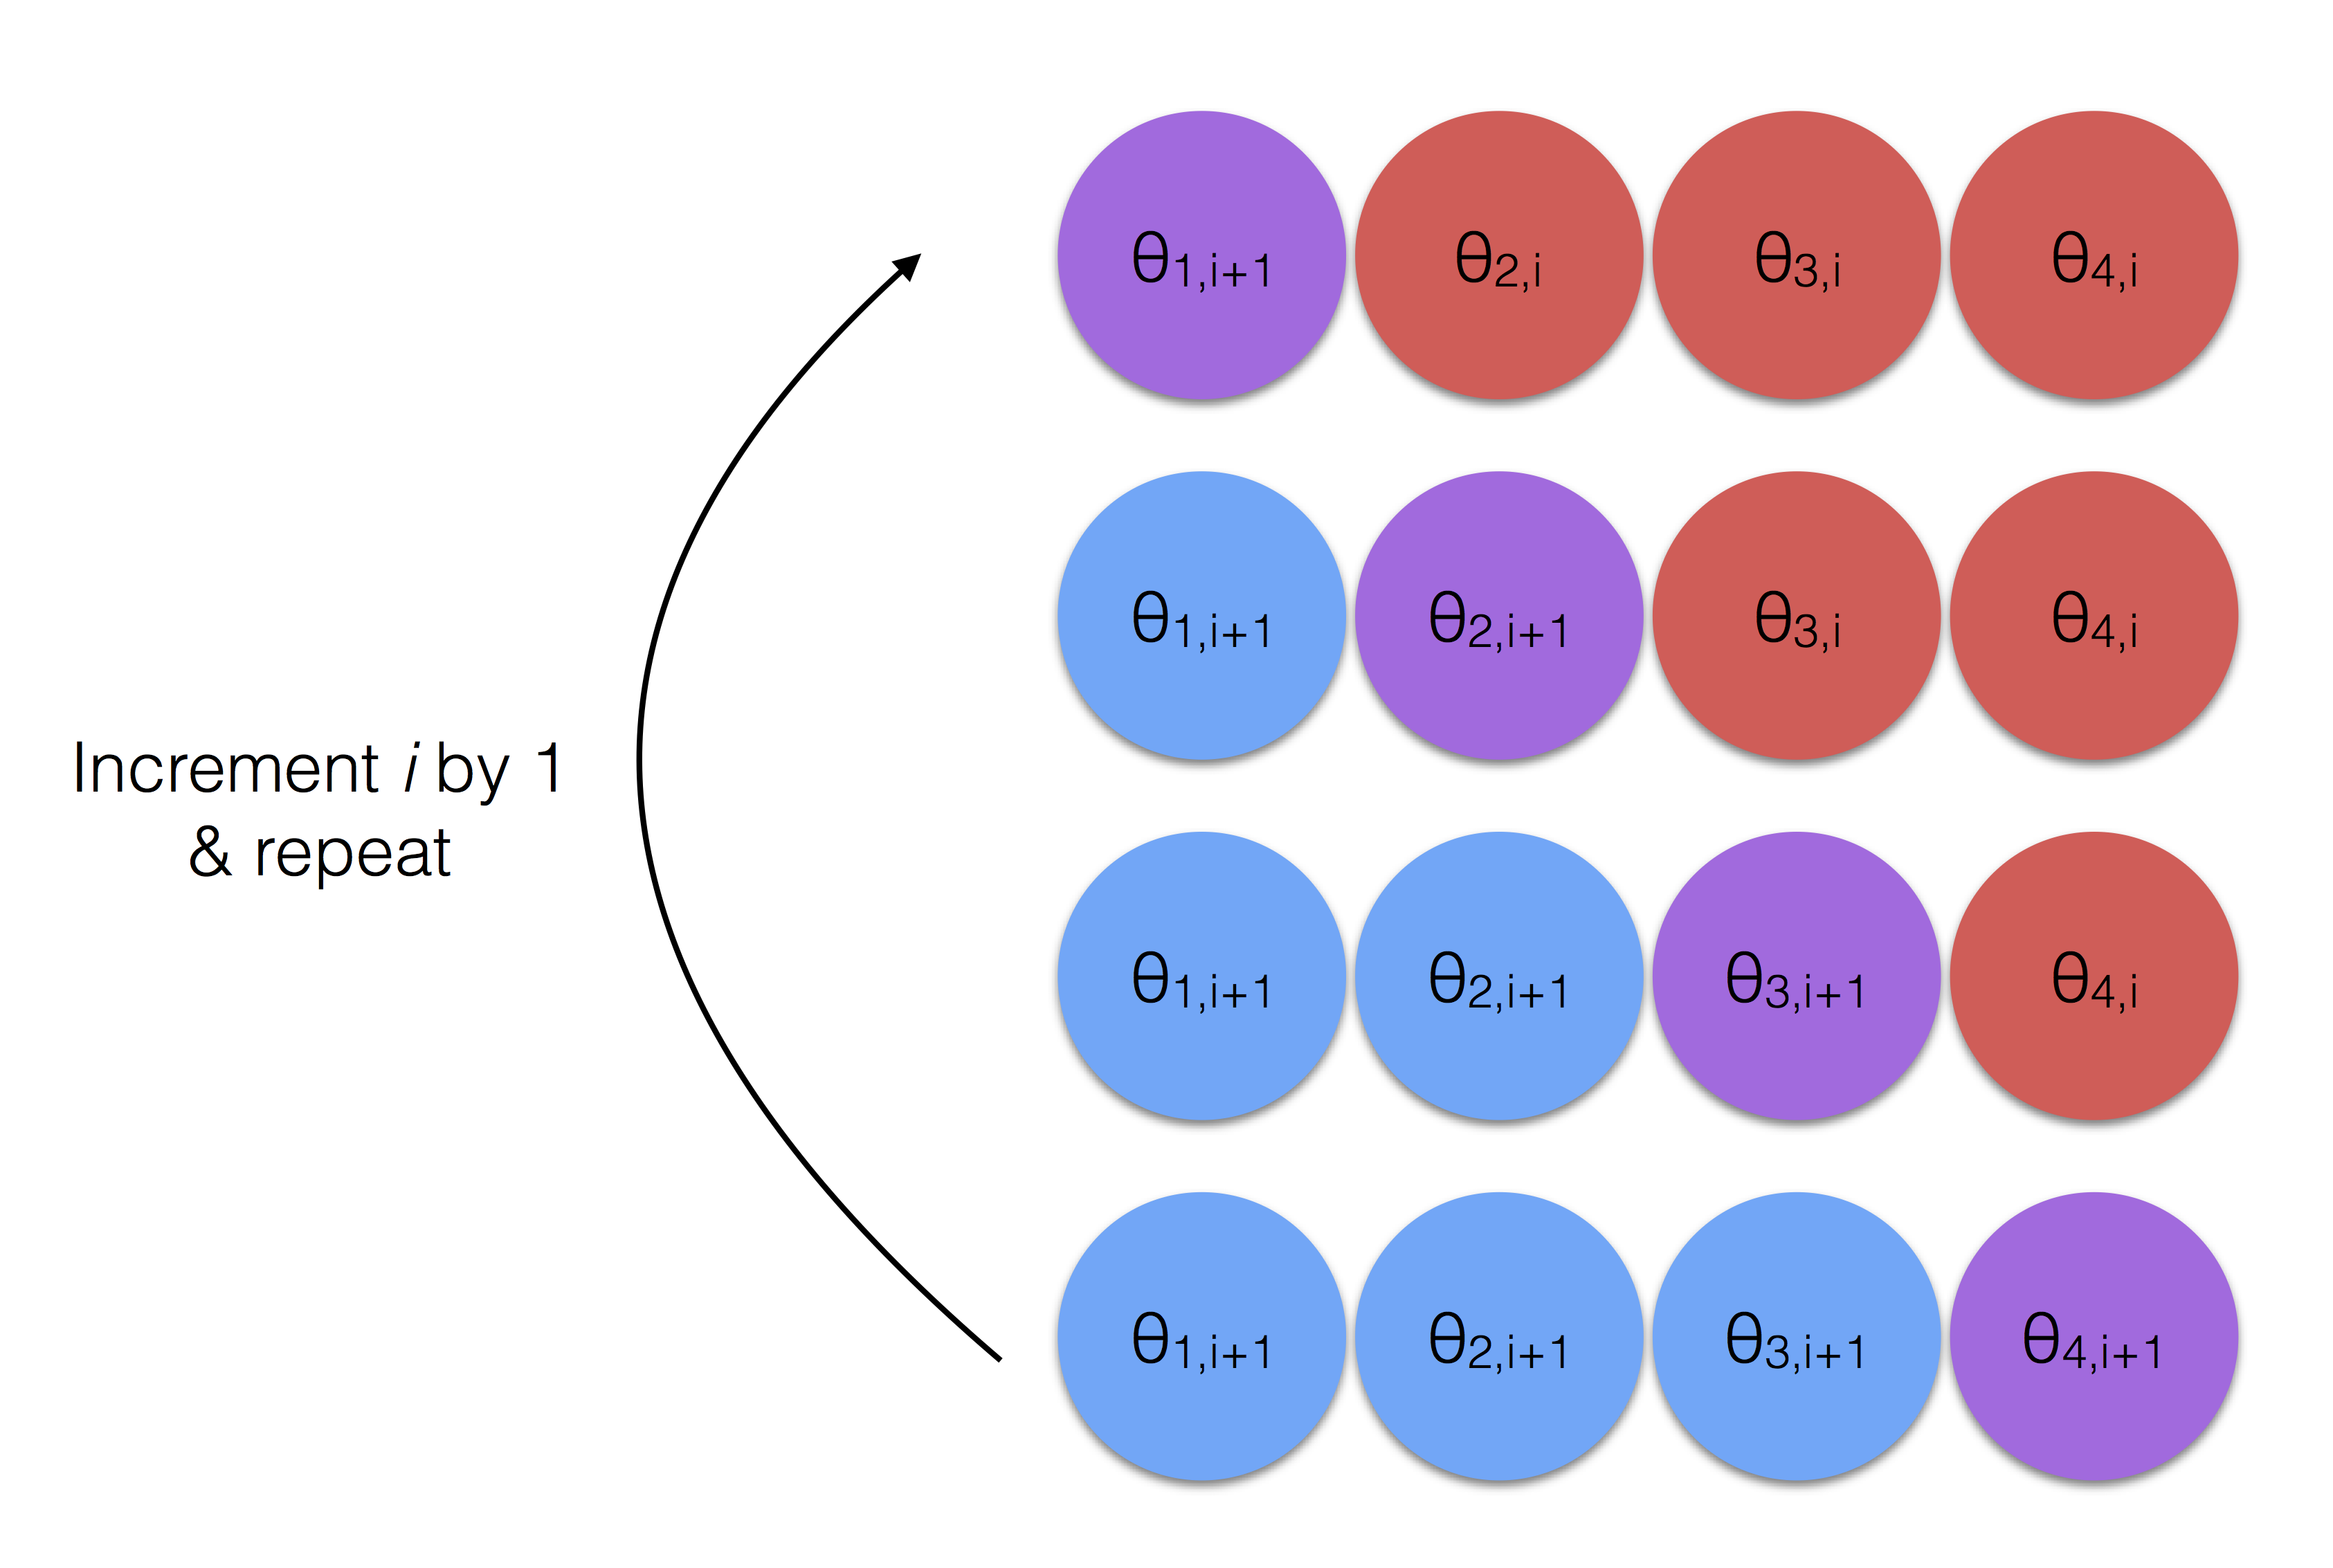
\includegraphics[width=8cm,height=5cm]{figures/ldaFig2_12_GibbsSamplingViz} \end{center}

\end{frame}

\begin{frame}{Base R Code}
\protect\hypertarget{base-r-code}{}

\begin{center}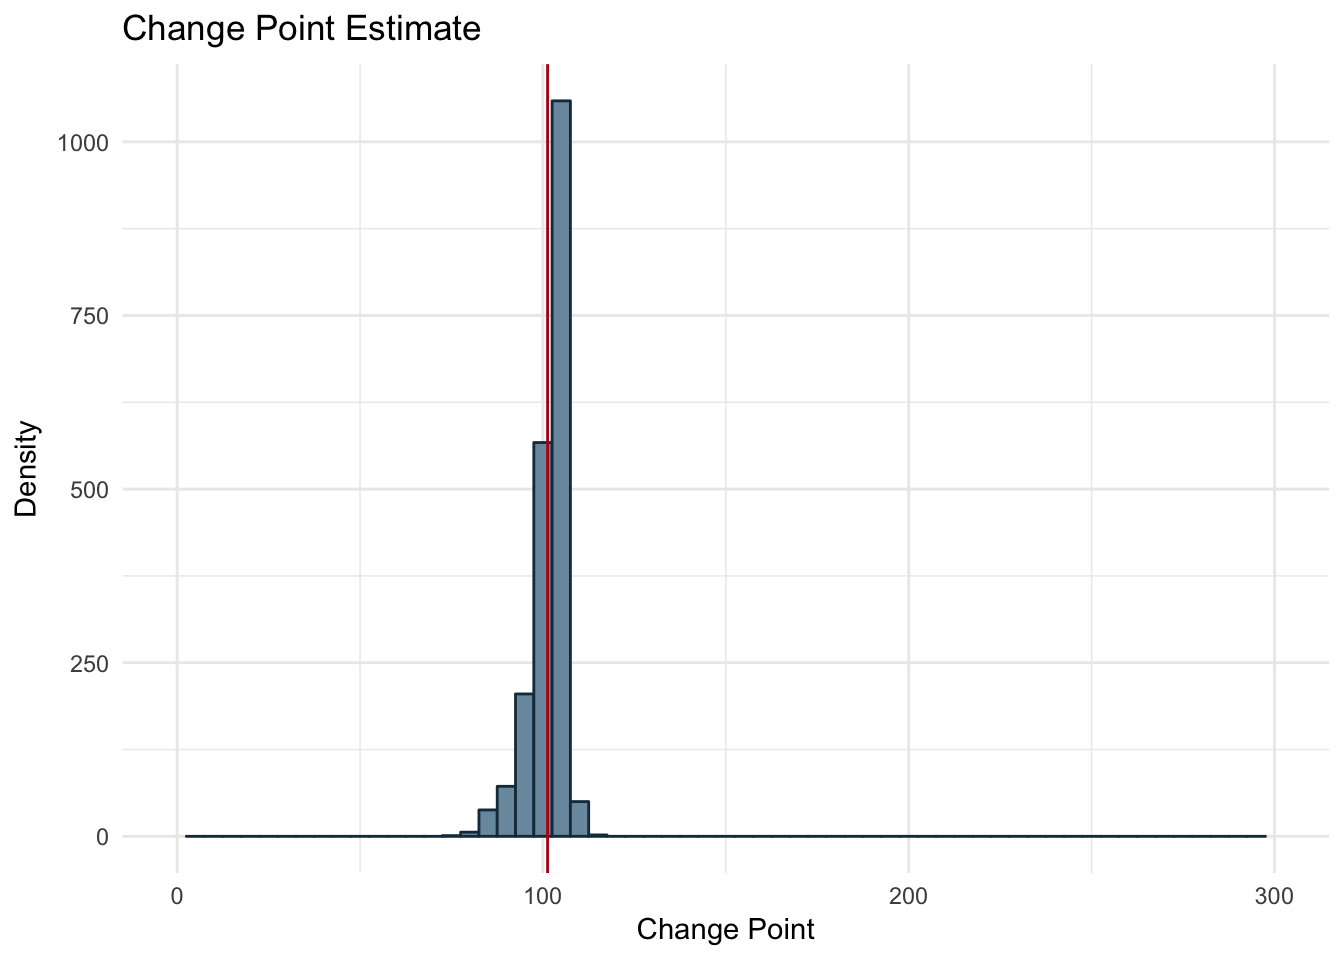
\includegraphics[width=8cm,height=6cm]{figures/ldaFig2_16_bernChangePointN-1} \end{center}

\end{frame}

\begin{frame}{Latent Variables}
\protect\hypertarget{latent-variables}{}

\footnotesize

The above task is trivial if one knew the value of \(n\) beforehand. In
fact, a human would eye-ball the change point and quickly compute the 2
separate means.

In machine learning, we would say that there is a
\textit{latent variable} (\(n\)) which is missing but knowledge of which
greatly simplifies the problem!

Instead of viewing the above as a change point detection, the task can
be phrased as a clustering problem: find the best partition into 2
groups.

Let us briefly review the most basic clustering algorithm.

\end{frame}

\begin{frame}{K-means Clustering}
\protect\hypertarget{k-means-clustering}{}

One chooses the desired number of cluster centers, say R, and the
K-means procedure iteratively moves the centers to minimize the total
within cluster variance. Given an initial set of centers, the K-means
algorithm alternates the two steps:

\begin{enumerate}
  \item for each center we identify the subset of training points (its cluster) that is closer to it than any other center;
  \item  the means of each feature for the data points in each cluster are
computed, and this mean vector becomes the new center for that cluster.
\end{enumerate}

These two steps are iterated until convergence. Typically the initial
centers are R randomly chosen observations from the training data

\end{frame}

\begin{frame}{Iterative Procedure}
\protect\hypertarget{iterative-procedure}{}

\begin{center}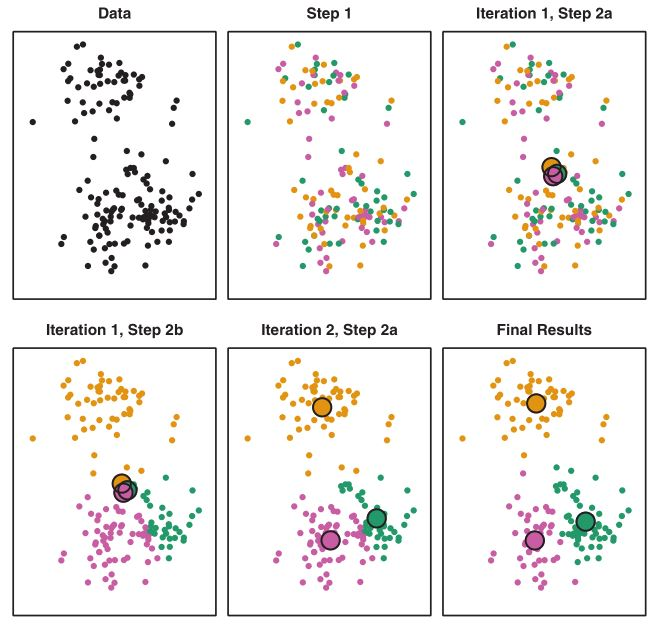
\includegraphics[height=7.5cm]{figures/ISLR_fig10-6_KMeans} \end{center}

\end{frame}

\hypertarget{the-em-algorithm}{%
\section{The EM Algorithm}\label{the-em-algorithm}}

\begin{frame}{Gaussian Mixtures as Soft K-means Clustering}
\protect\hypertarget{gaussian-mixtures-as-soft-k-means-clustering}{}

\footnotesize

Generative Model \begin{equation}
\begin{aligned}
Y_1 &\propto N(\mu_1,\sigma_1)\\
Y_2 &\propto N(\mu_2,\sigma_2)\\
Y &= \Delta \cdot Y_1 + (1- \Delta) \cdot Y_2 
\end{aligned}
\end{equation} Direct maximization of likelihood is difficult
numerically, but if we knew the \textbf{unobserved latent} variables
\(\Delta\), it would be simple.

\begin{center}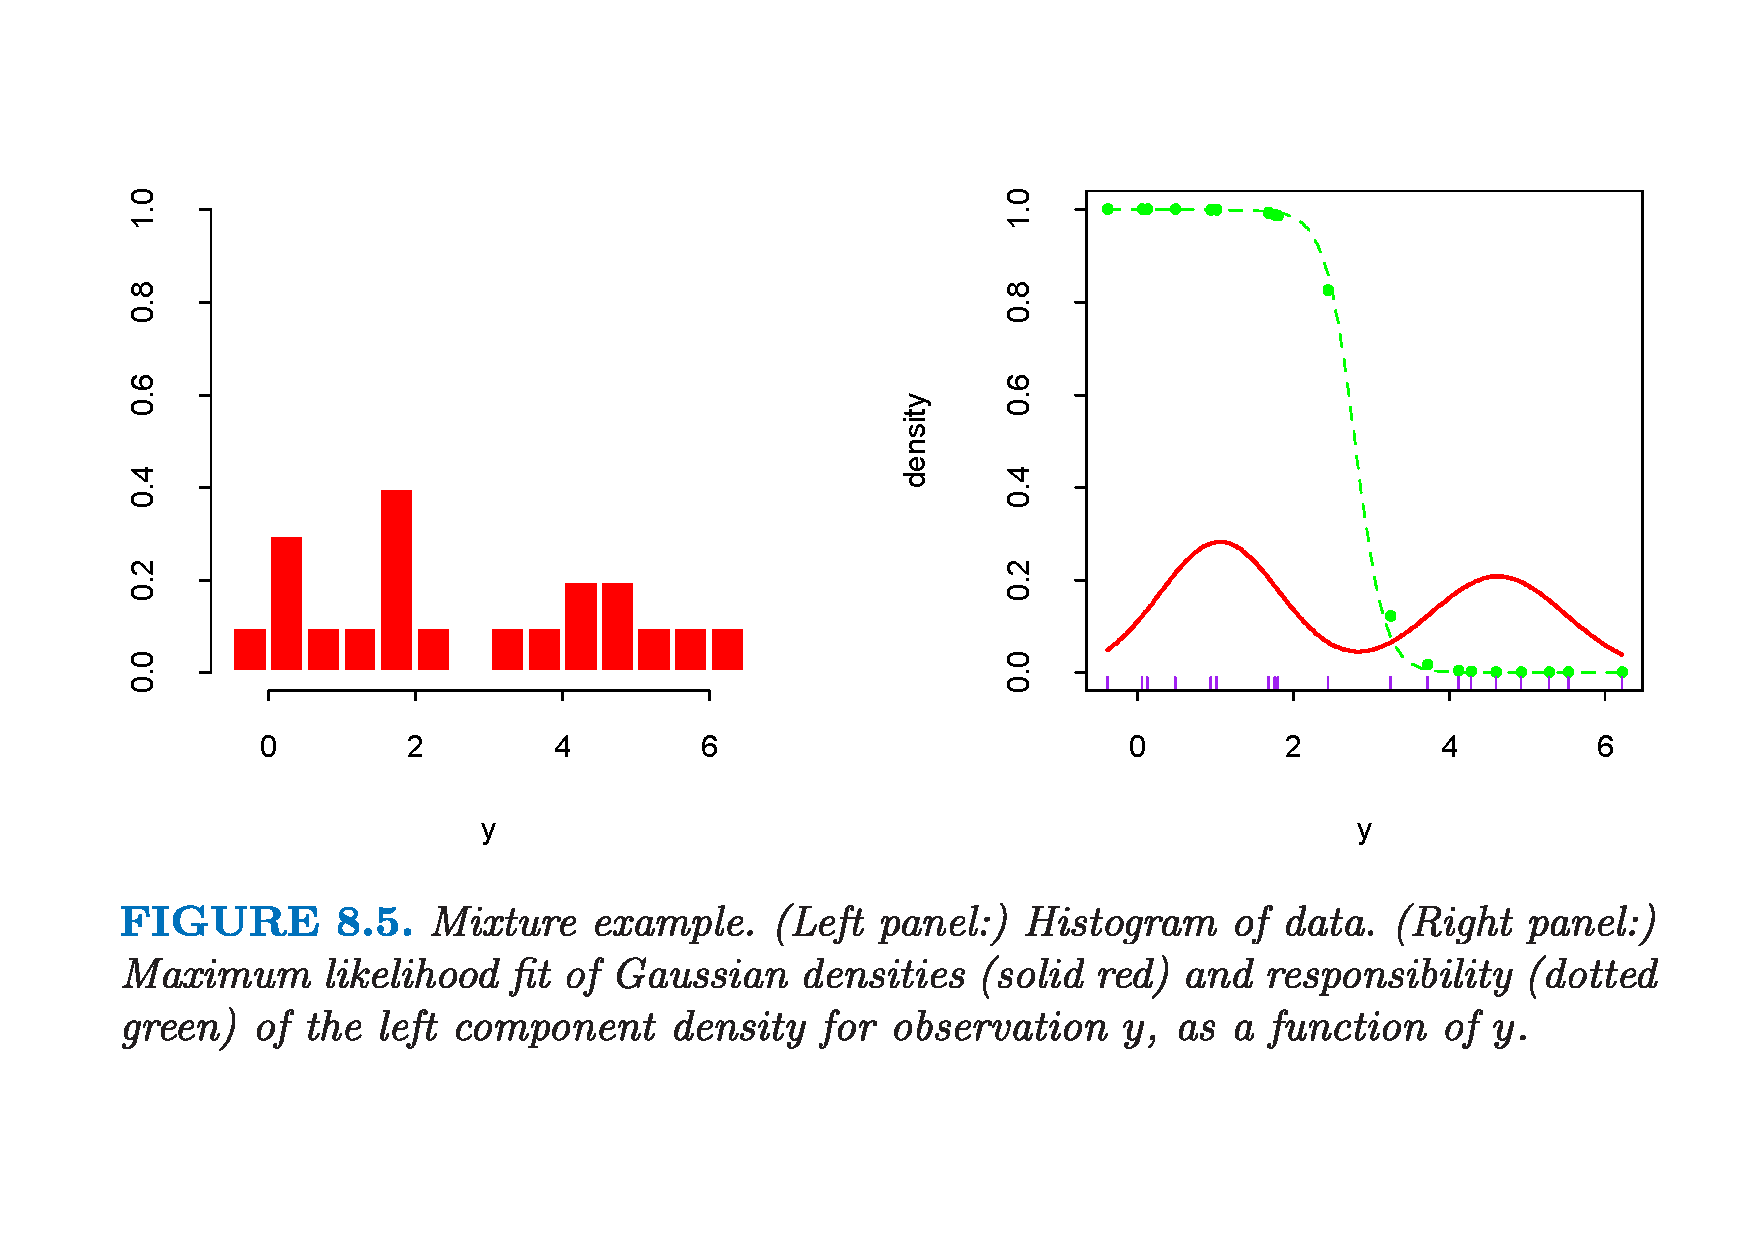
\includegraphics[height=5cm]{figures/ESL-Fig8-5} \end{center}

\end{frame}

\begin{frame}{The EM algorithm}
\protect\hypertarget{the-em-algorithm-1}{}

\begin{center}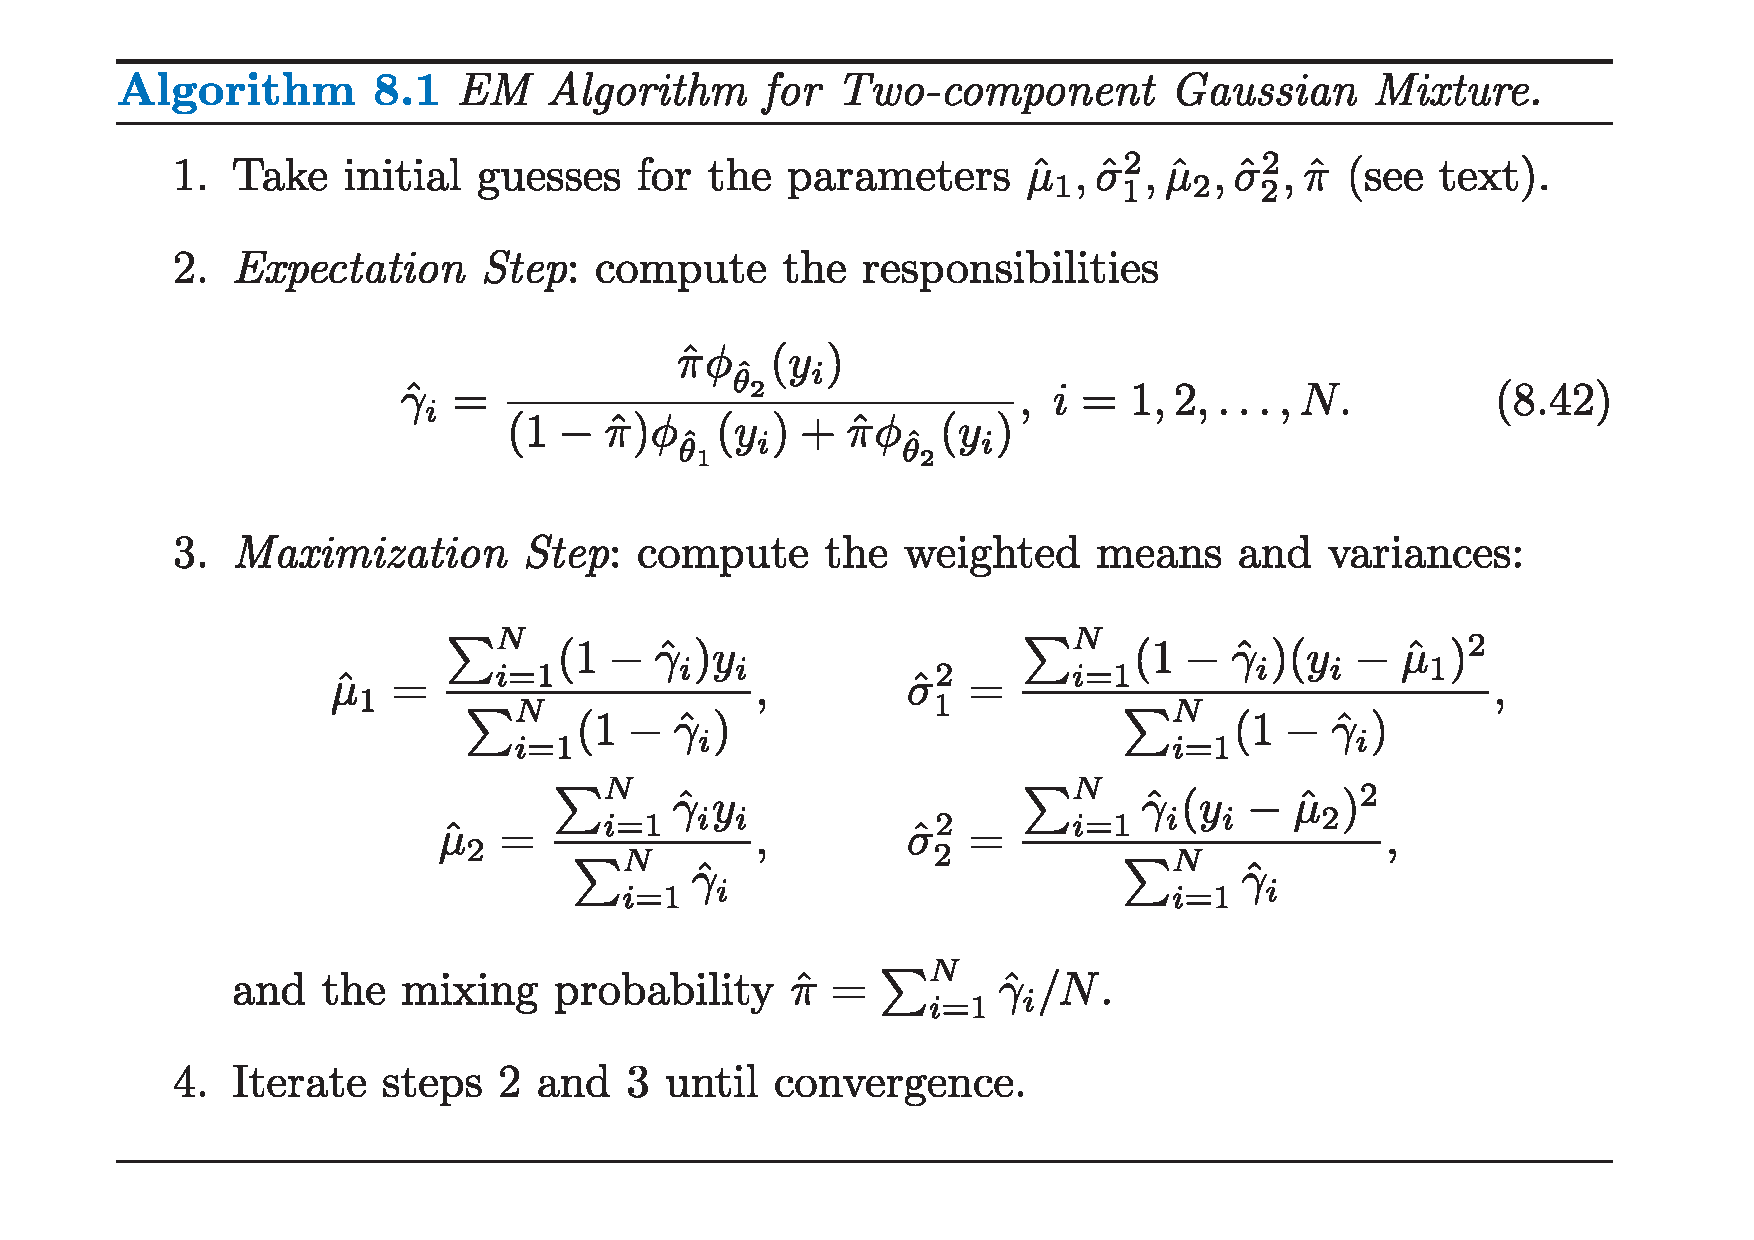
\includegraphics[height=7cm]{figures/ESL-Alg8-1} \end{center}

\end{frame}

\begin{frame}{Gibbs and EM}
\protect\hypertarget{gibbs-and-em}{}

Gibbs sampling is closely related to the EM algorithm: the main
difference is that it samples from the conditional distributions rather
than maximizing over them.

\begin{center}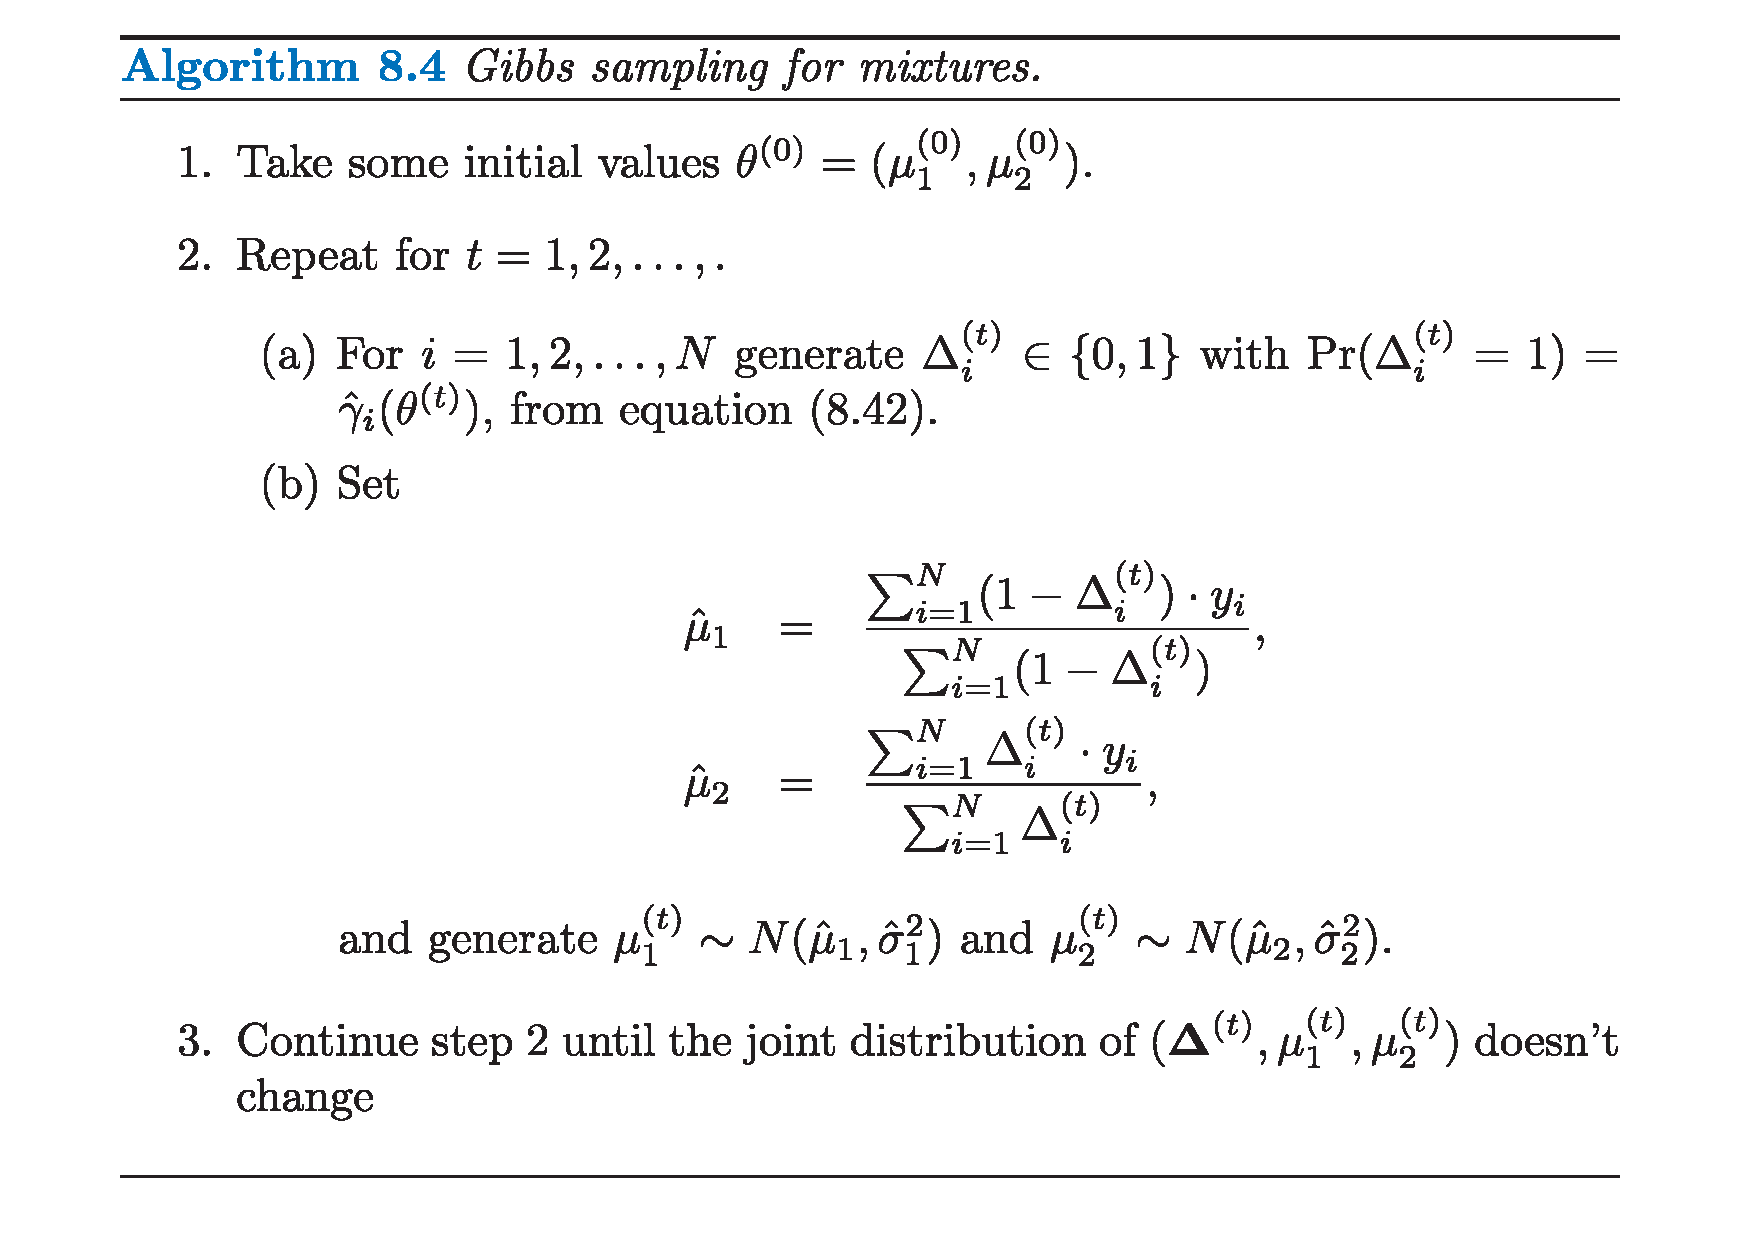
\includegraphics[height=7cm]{figures/ESL-Alg8-4} \end{center}

\end{frame}

\begin{frame}{Gibbs and EM, details}
\protect\hypertarget{gibbs-and-em-details}{}

\footnotesize

The key is to consider the latent data \(Z^m\) from the EM procedure to
be another parameter for the Gibbs sampler. To make this explicit for
the Gaussian mixture problem, we take our parameters to be
\((\theta, Z^m)\). For simplicity we fix the variances
\(\sigma_1^2,\sigma_2^2\) and mixing proportion \(\pi\) at their maximum
likelihood values so that the only unknown parameters in \(\theta\) are
the means \(\mu_1\) and \(\mu_2\). The Gibbs sampler for the mixture
problem is given in Algorithm 8.4.

We see that steps 2(a) and 2(b) are the same as the E and M steps of the
EM procedure, except that we sample rather than maximize. In step 2(a),
rather than compute the maximum likelihood responsibilities
\(\gamma_i = E(\Delta_i | \theta, Z^m)\), the Gibbs sampling procedure
simulates the latent data \(\Delta_i\) from the distributions
\(Pr(\Delta_i | \theta, Z^m)\). In step 2(b), rather than compute the
maximizers of the posterior \(Pr(\mu_1, \mu_2, \Delta |Z )\) we simulate
from the conditional distribution \(Pr(\mu_1, \mu_2, \Delta |Z )\).

\end{frame}

\hypertarget{multinomial}{%
\section{Multinomial}\label{multinomial}}

\begin{frame}{Multinomial \textless{}-\textgreater{} Dirichlet}
\protect\hypertarget{multinomial---dirichlet}{}

\footnotesize

\textbf{How Multinomial and Bernoulli Relate}

\begin{equation}
f(x)=\dfrac{n!}{x_1!x_2!\cdots x_K!}\theta_1^{x_1} \theta_2^{x_2} \cdots \theta_k^{x_K}
\end{equation}

The \textbf{conjugate prior} for the multinomial distribution is the
\textbf{Dirichlet} distribution. Similar to the beta distribution,
Dirichlet can be thought of as a distribution of distributions. Also
note that the beta distribution is the special case of a Dirichlet
distribution where the number of possible outcomes is 2. This is similar
to the relationship between the binomial and multinomial distributions.

\begin{equation}
Dir(\overrightarrow{\theta}|\overrightarrow{\alpha})=
{ 
  {\Gamma {\bigl (}\sum _{i=1}^{K}\alpha _{i}{\bigr )}}
  \over{\prod _{i=1}^{K}\Gamma (\alpha _{i})}
}
\prod _{i=1}^{K}\theta_{i}^{\alpha _{i}-1} =
{ 
  1 \over B(\alpha)
}
\prod _{i=1}^{K}\theta_{i}^{\alpha _{i}-1} 
\end{equation}

\end{frame}

\begin{frame}{Sampling from Dirichlet}
\protect\hypertarget{sampling-from-dirichlet}{}

\footnotesize

The distribution of samples for each category (\(\alpha_{i}\) value),
are approximately centered at the ratio of the \(\alpha_{i}\) value to
the sum of all \(\alpha\) values.

\begin{center}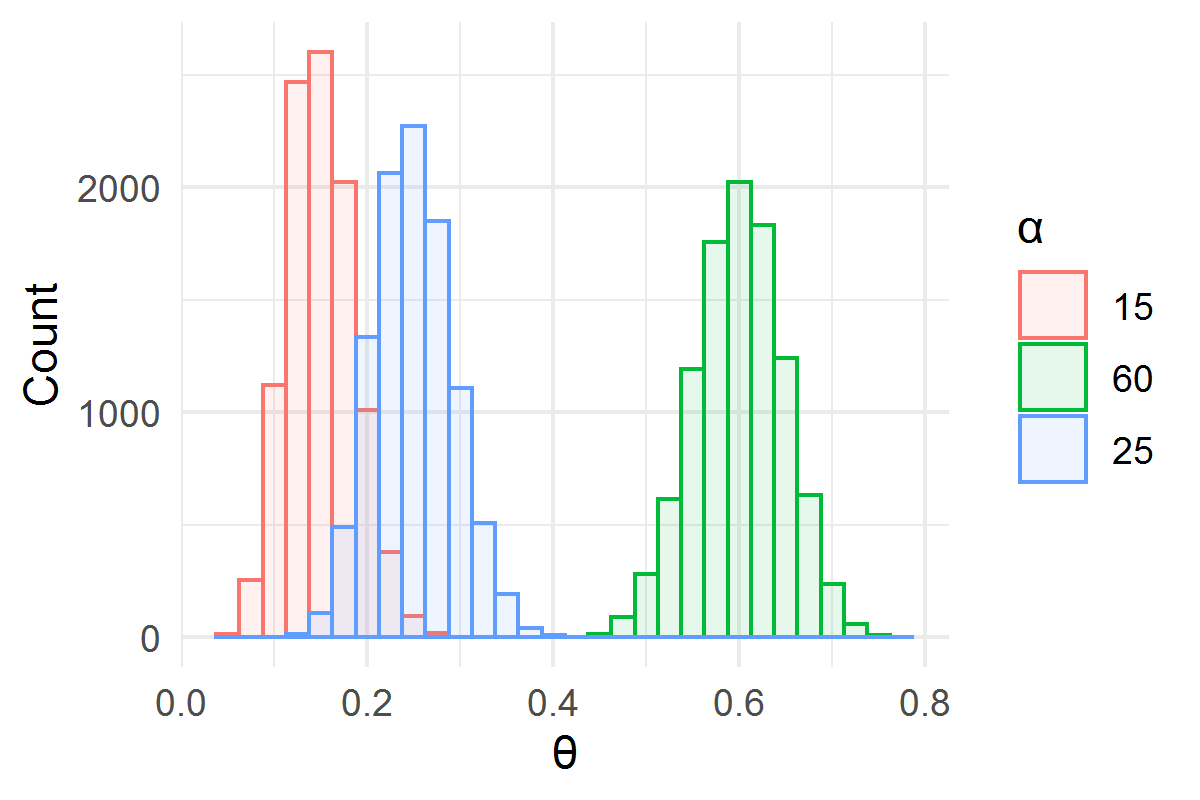
\includegraphics[width=6cm,height=4cm]{figures/DirchletSamples1} \end{center}

This is similar to the shift of the beta distribution when using
hyperparameters that are unequal.

\end{frame}

\begin{frame}{Dirichlet - Multinomial}
\protect\hypertarget{dirichlet---multinomial}{}

\footnotesize

The multinomial distribution with parameters
\(\overrightarrow{\theta} = \theta_{1}, \theta_{2}, ... \theta_{n}\) for
words \(1\) to \(n\) would be capable of generating a bag of words (BOW)
representation of a document. The model will be used to generate a
document using a limited vocabulary, only 3 distinct words:
\(\color{blue} \Delta, \color{red} \Omega, \color{darkgreen} \Psi\)., in
particular using the word counts as our \(\alpha\) values for the
dirichlet prior. \(\color{blue} \Delta\) \(\color{blue} \Delta\)
\(\color{blue} \Delta\) \(\color{blue} \Delta\) \(\color{blue} \Delta\)
\(\color{blue} \Delta\) \(\color{blue} \Delta\) \(\color{blue} \Delta\)
\(\color{red} \Omega\) \(\color{darkgreen} \Psi\)

Then we use the \(\theta\) values generated by the dirichlet prior as
the parameters for a multinomial distribution to generate the next term
in the document.

1 \(\color{blue} \Delta\) \(\color{blue} \Delta\)
\(\color{darkgreen} \Psi\) \(\color{blue} \Delta\)
\(\color{blue} \Delta\) \(\color{red} \Omega\) \(\color{blue} \Delta\)
\(\color{blue} \Delta\) \(\color{blue} \Delta\) \(\color{blue} \Delta\)
\newline2 \(\color{darkgreen} \Psi\) \(\color{blue} \Delta\)
\(\color{red} \Omega\) \(\color{blue} \Delta\) \(\color{blue} \Delta\)
\(\color{darkgreen} \Psi\) \(\color{blue} \Delta\)
\(\color{blue} \Delta\) \(\color{red} \Omega\) \(\color{blue} \Delta\)
\newline3 \(\color{blue} \Delta\) \(\color{blue} \Delta\)
\(\color{blue} \Delta\) \(\color{blue} \Delta\) \(\color{red} \Omega\)
\(\color{blue} \Delta\) \(\color{blue} \Delta\) \(\color{red} \Omega\)
\(\color{blue} \Delta\) \(\color{blue} \Delta\) \newline4
\(\color{blue} \Delta\) \(\color{darkgreen} \Psi\)
\(\color{blue} \Delta\) \(\color{darkgreen} \Psi\)
\(\color{blue} \Delta\) \(\color{blue} \Delta\) \(\color{red} \Omega\)
\(\color{red} \Omega\) \(\color{blue} \Delta\) \(\color{blue} \Delta\)
\newline5 \(\color{blue} \Delta\) \(\color{blue} \Delta\)
\(\color{blue} \Delta\) \(\color{darkgreen} \Psi\)
\(\color{blue} \Delta\) \(\color{darkgreen} \Psi\)
\(\color{blue} \Delta\) \(\color{blue} \Delta\) \(\color{blue} \Delta\)
\(\color{blue} \Delta\) \newline

\end{frame}

\begin{frame}{Inference I}
\protect\hypertarget{inference-i}{}

\footnotesize

The process above is a \textbf{generative model}. Now we are going to
take a series of pre-existing documents and infer what model created
them

Once we plug in the prior and likelihood and simplify, we find that we
are left with a Dirichlet PDF with the input parameters of
\(\overrightarrow{\alpha} + \overrightarrow{n}\) where \emph{n} are the
observed word counts.

\begin{equation}
\begin{aligned}
p(\theta|D) &\propto p(D|\theta)p(\theta)\\
&\propto \prod _{i=1}^{K}\theta^{n(k)} { 
  {\Gamma {\bigl (}\sum _{i=1}^{K}\alpha _{i}{\bigr )}}
  \over{\prod _{i=1}^{K}\Gamma (\alpha _{i})}
}
\prod _{i=1}^{K}\theta_{i}^{\alpha _{i}-1} \\
&\propto{ 
  {\Gamma {\bigl (}\sum _{i=1}^{K}\alpha _{i}{\bigr )}}
  \over{\prod _{i=1}^{K}\Gamma (\alpha _{i})}
}\prod _{i=1}^{K}\theta_{i}^{\alpha _{i}+n_{k}-1} \\
&\propto Dir(\overrightarrow{\alpha} + \overrightarrow{n})
\end{aligned}
\end{equation}

\end{frame}

\begin{frame}{Inference II}
\protect\hypertarget{inference-ii}{}

Let's use the 5 documents we previously generated as our basis and infer
the parameters used to generate them via Gibbs sampling.

\begin{center}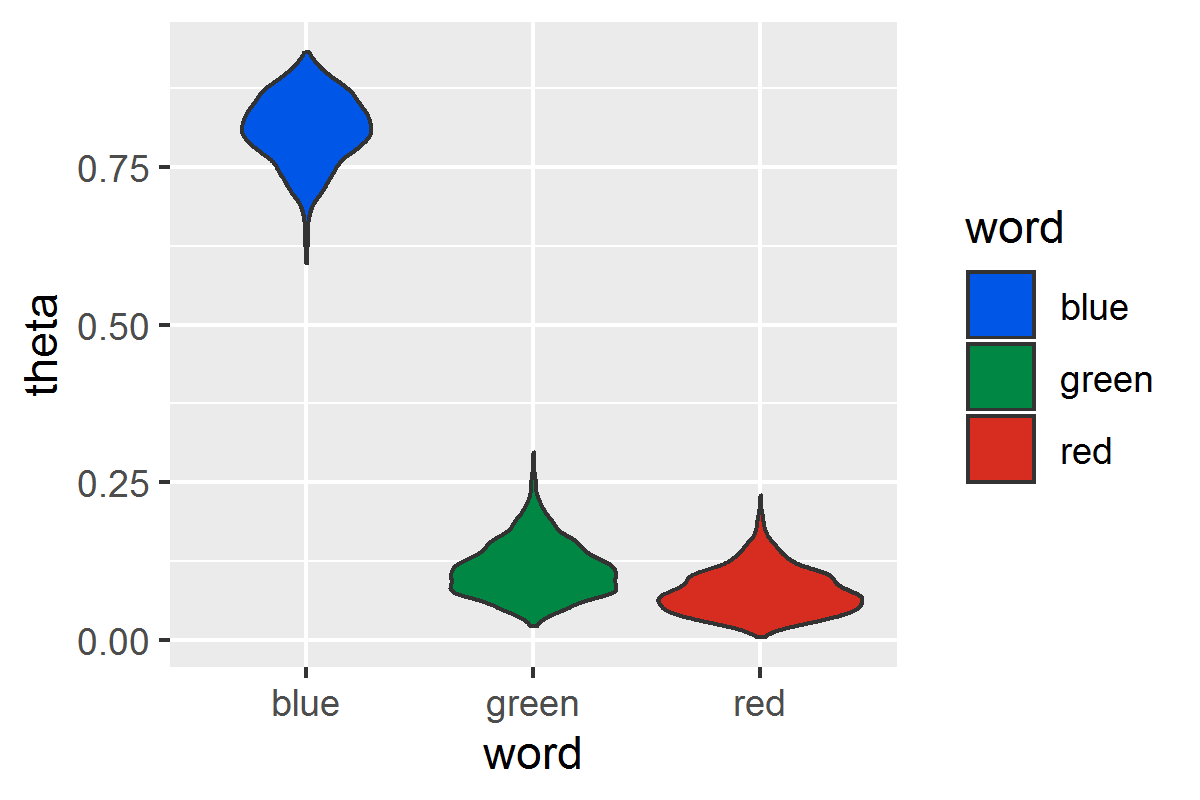
\includegraphics[width=8cm,height=6cm]{figures/unigramInference10} \end{center}

\end{frame}

\begin{frame}{Inference III}
\protect\hypertarget{inference-iii}{}

Instead of just 5 documents we will generate 500 and use this as our
sample to infer the word mixtures from.

\begin{center}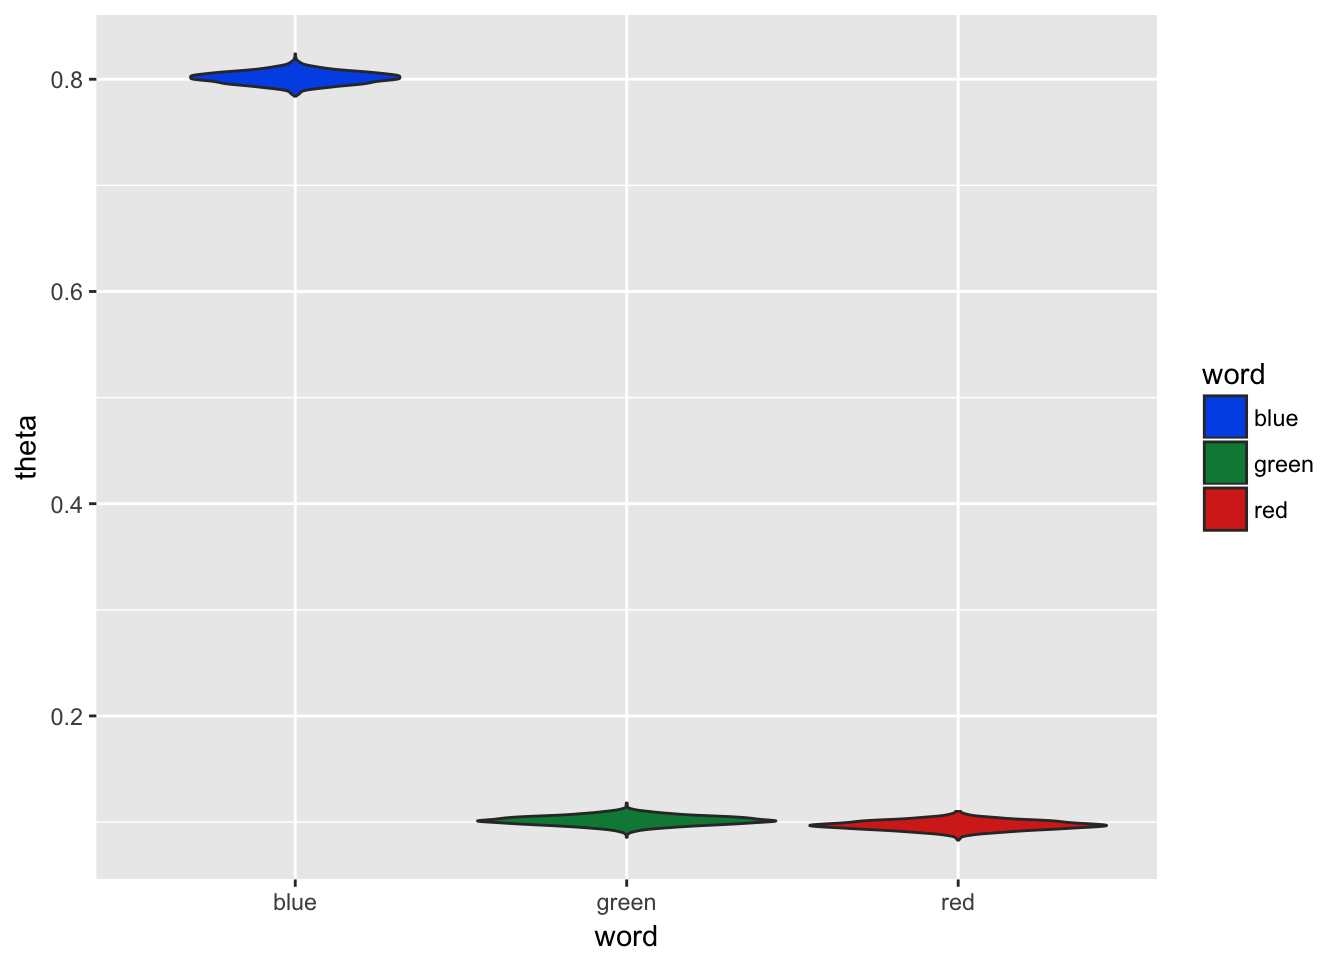
\includegraphics[width=8cm,height=6cm]{figures/unigramInference500} \end{center}

\end{frame}

\hypertarget{lda}{%
\section{LDA}\label{lda}}

\begin{frame}{Latent Dirichlet allocation}
\protect\hypertarget{latent-dirichlet-allocation}{}

\footnotesize

Latent Dirichlet allocation is one of the most common algorithms for
topic modeling. It is guided by two principles.

\begin{itemize}
\tightlist
\item
  \textbf{Every document is a mixture of topics.} We imagine that each
  document may contain words from several topics in particular
  proportions. For example, in a two-topic model we could say ``Document
  1 is 90\% topic A and 10\% topic B, while Document 2 is 30\% topic A
  and 70\% topic B.''
\item
  \textbf{Every topic is a mixture of words.} For example, we could
  imagine a two-topic model of American news, with one topic for
  ``politics'' and one for ``entertainment.'' The most common words in
  the politics topic might be ``President'', ``Congress'', and
  ``government'', while the entertainment topic may be made up of words
  such as ``movies'', ``television'', and ``actor''. Importantly, words
  can be shared between topics; a word like ``budget'' might appear in
  both equally.
\end{itemize}

\end{frame}

\begin{frame}{Mixture of Words \textbf{and} Topics}
\protect\hypertarget{mixture-of-words-and-topics}{}

\footnotesize

\begin{itemize}
\tightlist
\item
  \textbf{Documents (d in D):}, that we want to identify the topic
  structures of.
\item
  \textbf{Words (w in W):} We have a collection of words and word counts
  for each document.
\item
  \textbf{Hyperparameters:}

  \begin{itemize}
  \tightlist
  \item
    \(\overrightarrow{\alpha}\): Our prior assumption about the topic
    distribution of our documents. We will be supplying the \(\alpha\)
    value for inference.

    \begin{itemize}
    \tightlist
    \item
      Higher \(\overrightarrow{\alpha}\) - We assume documents will have
      a similar and close to uniform distribution of topics.
    \item
      Lower \(\overrightarrow{\alpha}\) - We assume document topic
      distributions vary more drastically.
    \end{itemize}
  \item
    \(\overrightarrow{\beta}\): Our prior assumption about the word
    distribution of each topic.

    \begin{itemize}
    \tightlist
    \item
      Higher \(\overrightarrow{\beta}\): Word distributions in each
      topic are closer to uniform, i.e.~each word is equally as likely
      in each topic.
    \item
      Lower \(\overrightarrow{\beta}\): Word distributions vary more
      from topic to topic.
    \end{itemize}
  \end{itemize}
\end{itemize}

\end{frame}

\begin{frame}{Simplified View}
\protect\hypertarget{simplified-view}{}

\footnotesize
\begin{itemize}
\item Go through each document $d$, and randomly assign each word in the document to one of the $K$ topics.
\item For each document $d$, 
   \begin{itemize}
      \item For each word $w$ in $d$, and each topic $t$, compute: 
      \begin{enumerate}
        \item $p( t |  d)$ =  proportion of words in document $d$ that are currently assigned to topic $t$, and        
        \item $p( w |  t)$ =  proportion of assignments to topic $t$ over all documents that come from this word $w$.
        \item Reassign $w$ a new topic $t$ with the probability that topic $t$ generated word $w$: $p( t |  d) \cdot p( w |  t)$
      \end{enumerate}
    \end{itemize}   
\end{itemize}

In the last step, we're assuming that all topic assignments except for
the current word in question are correct, and then updating the
assignment of the current word using our model of how documents are
generated.

\end{frame}

\begin{frame}{Gibbs Sampling}
\protect\hypertarget{gibbs-sampling-2}{}

The main goal of inference in LDA is to determine the topic of each word
\(w\), \(z_{i}\) (topic of word \emph{i}), in each document:
\(p(z_{i}|z_{\neg i}, \alpha, \beta, w)\).

\begin{equation}
\begin{aligned}
p(z_{i}|z_{\neg i}, w) & \propto \overbrace{ {n_{d,\neg i}^{k} + \alpha_{k} \over 
  \sum_{k} n_{d,\neg i}^{k} + \alpha_{k}} }^{document-topic} \cdot \overbrace{ {n_{k,\neg i}^{w} + \beta_{w} \over 
  \sum_{w} n_{k,\neg i}^{w} + \beta_{w}}}^{topic-word} 
\end{aligned}
\end{equation}

where

\begin{itemize}
\item
  \(n_{d,\neg i}^{k}\): Number of times document \(d\) use topic \(k\)
\item
  \(n_{k,\neg i}^{w}\): Number of times topic k uses the given word
\end{itemize}

\end{frame}

\hypertarget{software-references}{%
\section{Software \& References}\label{software-references}}

\begin{frame}{Software}
\protect\hypertarget{software}{}

\begin{itemize}
  \item The \textbf{OpenBUGS} software (Bayesian inference Using Gibbs Sampling) does a Bayesian analysis of complex statistical models using Markov chain Monte Carlo.

   \item  \textbf{JAGS} (Just another Gibbs sampler) is a GPL program for analysis of Bayesian hierarchical models using Markov Chain Monte Carlo.

  \item \textbf{PyMC3} is an open source Python library for Bayesian learning of general Probabilistic Graphical Model with advanced features and easy to use interface.

  \item \textbf{Turing} is a Julia package that allows multiple sampler types to be run as components of Gibbs sampling. 

\end{itemize}

\end{frame}

\begin{frame}{RJAGS}
\protect\hypertarget{rjags}{}

\end{frame}

\begin{frame}{Closing Remarks}
\protect\hypertarget{closing-remarks}{}

\footnotesize

\begin{itemize}
\item
  Generally, samples from the beginning of the chain (the burn-in
  period) may not accurately represent the desired distribution and are
  usually discarded.
\item
  A \textbf{blocked Gibbs sampler} groups two or more variables together
  and samples from their joint distribution conditioned on all other
  variables, rather than sampling from each one individually.
\item
  A \textbf{collapsed Gibbs sampler} integrates out (marginalizes over)
  one or more variables when sampling for some other variable.
\item
  Failure modes:

  \begin{itemize}
  \tightlist
  \item
    islands of high-probability states, with no paths between them
  \item
    all states have nonzero probability and there is only a single
    island of high-probability states
  \end{itemize}
\end{itemize}

\end{frame}

\begin{frame}{Further References}
\protect\hypertarget{further-references}{}

\begin{itemize}

  \item  \href{http://users.umiacs.umd.edu/~jbg/}{\color{blue}{Jordan Boyd Graber at UMD}}: 
 \begin{itemize}
      \item   Videos, e.g. \href{https://www.youtube.com/watch?v=u7l5hhmdc0M}{\color{blue}{Topic Models: Gibbs Sampling}} or \href{https://www.youtube.com/watch?v=CEVELIz4WXM}{\color{blue}{Beta and Dirichlet Distributions}} or \href{https://www.youtube.com/watch?v=0NMC2NfJGqo}{\color{blue}{Clustering: Gaussian Mixture Models}} 
    
  \item \href{https://github.com/ezubaric/TM_applications_book}{\color{blue}{book}} on Applications of Topic Models
  \end{itemize}
  \item  \href{https://ldabook.com}{\color{blue}{The Little LDA book}}
  
  
  \item  \href{https://web.stanford.edu/~hastie/Papers/ESLII}{\color{blue}{The Elements of Statistical Learning}} 
  \item    \href{http://topicmodels.west.uni-koblenz.de/}{\color{blue}{Uni Koblenz}}, e.g. \href{http://topicmodels.west.uni-koblenz.de/ckling/tmt/restaurant.html?parameters=1\%2C2\%2C1\%2C2\%2C1\%2C3\#}{\color{blue}{Animation Polya urn}} 

  \item    \href{https://www.tidytextmining.com/}{\color{blue}{Tidy Text Mining}}, chapter 6
\end{itemize}

\end{frame}

\end{document}
